\chapter{勒贝格积分}

前言中介绍了黎曼积分存在的某些缺陷, 这些缺陷限制了黎曼积分的应用. 二十世纪初,
法国数学家勒贝格~(1875--1941)~创建了一种新的勒贝格积分理论.

勒贝格积分是在勒贝格测度理论的基础上建立起来的, 这一理论可以统一处理函数有界和无界的情形. 黎曼积分通常讨论的是闭区间~$[a,\, b]$~上的函数, 而勒贝格积分定义域可以是更一般的点集即可测集. 更重要的是, 它提供了比黎曼积分更广泛而有用的收敛定理.

本章先由简单函数的勒贝格积分入手, 然后到非负可测函数, 再到一般可测函数的勒贝格积分; 并讨论了勒贝格积分的性质, 特别是列维定理, 法都引理与勒贝格控制收敛定理; 另外, 进一步发掘黎曼积分和勒贝格积分内在联系, 并给出黎曼可积函数的一个判别条件.

\section{勒贝格积分的定义}

\subsection{非负简单函数的勒贝格积分}

\begin{definition}
设~$f(x)$~为~$E$~上的非负简单函数, 记~$f(x) = \sum\limits_{i=1}^n a_i \chi_{E_i}(x)$,  其中~$E_i$~可测、互不相交, 且~$\smallcup\limits_{i=1}^n E_i = E$, 定义
\[
(L)\int_E f(x) \d \mu = \sum_{i=1}^n a_i m(E_i)
\]
称为~$f(x)$~在~$E$~上(关于测度~$m$~)的勒贝格积分.
\end{definition}

\begin{remark}
(1) $\int_E f(x) \d \mu$~可以是~$+\infty$.

\vspace{0.5ex}

(2) $\int_E f(x) \d \mu = \int_{\mathbb{R}^n} f(x) \chi_E (x) \d \mu$.

\vspace{0.5ex}

(3) 数值~$\int_E f(x) \d \mu$~是确定的, 即不依赖于~$f$~表达式的选取.
\end{remark}


\begin{lemma} \label{lem410}
设~$f(x)=\sum\limits_{i=1}^n a_i \chi_{E_i}(x)$, $g(x)=\sum\limits_{j=1}^m b_j \chi_{e_j}(x)$~为~$E$~上的简单函数，则它们可以表示为统一形式：
\[
f(x)=\sum\limits_{i=1}^n \sum\limits_{j=1}^m a_i \chi_{E_i \cap e_j}(x), \qquad g(x)= \sum\limits_{i=1}^n \sum\limits_{j=1}^m b_j \chi_{E_i \cap e_j}(x)
\]
实际上，对于~$E$~的两种划分：$E=\mathop{\smallcup}\limits_{i=1}^n E_i=\mathop{\smallcup}\limits_{j=1}^m e_j$, 其中，$E_i$~互不相交，$e_j$~互不相交。则
\[
E=\mathop{\smallcup}\limits_{i=1}^n E_i = \mathop{\smallcup}\limits_{i=1}^n (E_i \cap E) = \mathop{\smallcup}\limits_{i=1}^n \Big(E_i \cap \mathop{\smallcup}\limits_{j=1}^m e_j \Big) =\mathop{\smallcup}\limits_{i=1}^n \mathop{\smallcup}\limits_{j=1}^m (E_i \cap e_j)
\]
显然，$(E_i \cap e_j)$~互不相交，且包含于~$E_i$~和~$e_j$, 故结论成立。
\end{lemma}

\begin{proof}
设~$f(x) = \sum\limits_{j=1}^m b_j \chi_{e_j}(x)$~为~$f$~的又一表达式, 则由引理~\ref{lem410}~知
\[
f(x)=\sum\limits_{i=1}^n \sum\limits_{j=1}^m a_i \chi_{E_i \cap e_j}(x) = \sum\limits_{i=1}^n \sum\limits_{j=1}^m b_j \chi_{E_i \cap e_j}(x)
\]
注意到，在~$(E_i \cap e_j)$~上有~$a_i=b_j$, 从而
\[
\int_E f(x) \d \mu = \sum_{i=1}^n \sum_{j=1}^m a_i m(E_i \cap e_j) = \sum_{i=1}^n \sum_{j=1}^m b_j m(E_i \cap e_j)
\]
因此, 非负简单函数勒贝格积分的定义有意义.
\end{proof}

\begin{example}
狄利克雷函数
\[
D(x) = \left\{ \!\!
\begin{array}{ll}
1,\, & x \mbox{~为~} [0,\, 1] \mbox{~上的有理数~} \\[0.1cm]
0,\, & x \mbox{~为~} [0,\, 1] \mbox{~上的无理数~}
\end{array}
\right.
\]
则~$D(x)$~的勒贝格积分
\[
(L)\int_{[0,1]} D(x) \d \mu = 1 \cdot m\big(\mathbb{Q}_{[0,1]}\big) + 0 \cdot m\big([0,\, 1] - \mathbb{Q}_{[0,1]} \big) = 0
\]
\end{example}

\begin{example}
设~$E \subset \mathbb{R}^n$~可测, 则
\[
\int_E 1 \d \mu = \int_{\mathbb{R}^n} \chi_E(x) \d \mu = m(E)
\]
\end{example}

\begin{proposition} \label{prop411}
设~$f(x),\,g(x)$~为~$E$~上的非负简单函数, 则

(i) $\int_E c f(x) \d \mu = c \int_E f(x) \d \mu, \, c \geqslant 0$~为实数;

(ii) $\int_E \big[f(x) + g(x)\big] \d \mu = \int_E f(x) \d \mu + \int_E g(x) \d \mu$;

(iii) 若~$f(x) \leqslant g(x),\, \mathrm{~a.e.~} x \in E$, 则~$\int_E f(x) \d \mu \leqslant \int_E g(x) \d \mu$.
\end{proposition}

\begin{proof}
(i) 显然成立.

(ii) 设~$f(x) = \sum\limits_{i=1}^n a_i \chi_{A_i}(x),\,g(x) = \sum\limits_{j=1}^m b_i \chi_{B_j}(x)$, 则由引理~\ref{lem410}~知
\[
f(x) = \sum\limits_{i=1}^n \sum\limits_{j=1}^m a_i \chi_{A_i \smallcap B_j} (x), \qquad g(x) = \sum\limits_{i=1}^n \sum\limits_{j=1}^m b_j \chi_{A_i \smallcap B_j} (x)
\]
从而
\[
f(x) + g(x) = \sum\limits_{i=1}^n \sum\limits_{j=1}^m (a_i + b_j) \chi_{A_i \smallcap B_j} (x)
\]
于是
\begin{eqnarray*}
\int_E [f(x)+g(x)] \d \mu &=& \sum_{i=1}^n \sum_{j=1}^m (a_i + b_j) m(A_i \medcap B_j) \\
&=& \sum_{i=1}^n \sum_{j=1}^m a_i m(A_i \medcap B_j) + \sum_{i=1}^n \sum_{j=1}^m b_j m(A_i \medcap B_j) \\
&=& \int_E f(x) \d \mu + \int_E g(x) \d \mu
\end{eqnarray*}

(iii) 由引理~\ref{lem410}, 不妨设~$f(x) = \sum\limits_{i=1}^n a_i \chi_{A_i}(x),\, g(x) = \sum\limits_{i=1}^n b_i \chi_{A_i}(x)$, 其中, $E = \mathop{\smallcup}\limits_{i=1}^n A_i$. 由于~$f(x) \leqslant g(x),\, \mathrm{~a.e.~} x \in E$, 则存在~$e \subset E,\, m(e) = 0$, 使得
\[
f(x) \leqslant g(x),\quad  \forall~x \in E - e
\]
由于
\[
A_i = A_i \medcap E = A_i \medcap \big((E-e) \medcup e\big) = \big(A_i \medcap (E-e)\big) \medcup (A_i \medcap e)
\]
故
\[
f(x) = \sum_{i=1}^n \big[ a_i \chi_{A_i \cap (E-e)}(x) + a_i \chi_{A_i \cap e}(x) \big]
\]
注意到~$m(A_i \smallcap e) = 0$, 从而
\begin{eqnarray*}
\int_E f(x) \d \mu &=& \sum_{i=1}^n \big[ a_i m\big(A_i \medcap (E-e)\big) + a_i m(A_i \medcap e) \big] \\
&\leqslant& \sum_{i=1}^n b_i m\big(A_i \medcap (E-e)\big) \\
&=& \sum_{i=1}^n \big[ b_i m\big(A_i \medcap (E-e)\big) + b_i m(A_i \medcap e) \big] \\
&=& \int_E g(x) \d \mu
\end{eqnarray*}
\end{proof}

\subsection{非负可测函数的勒贝格积分}

\begin{definition}
设~$f(x)$~为~$E$~上的非负可测函数, 定义
\[
(L)\int_E f(x) \d \mu = \sup \Big\{ \int_E \varphi(x) \d \mu: \: \varphi \mbox{~为~} E \mbox{~上简单函数且~} 0 \leqslant \varphi \leqslant f \Big\}
\]
称为~$f(x)$~在~$E$~上的勒贝格积分.
\end{definition}

\begin{theorem} \label{thm411}
设~$f(x)$~为~$E$~上的非负可测函数, 则存在单调递增的非负简单函数列~$\{f_n(x)\}$~使得
\[
\int_E f(x) \d \mu = \lim_{n \to \infty} \int_E f_n(x) \d \mu
\]
\end{theorem}

\begin{proof}
$f(x)$~在~$E$~上非负可测, 由可测函数构造定理, 存在单调递增的非负简单函数列~$\{f_n(x)\}$~使得
\[
f(x) = \lim\limits_{n \to \infty} f_n(x),\, \quad x \in E
\]
只需证明
\[
\lim_{n \to \infty} \int_E f_n(x) \d \mu = \sup \Big\{ \int_E \varphi(x) \d \mu: \: \varphi \mbox{~为~} E \mbox{~上简单函数且~} 0 \leqslant \varphi \leqslant f \Big\}
\]
显然, 左端~$\leqslant$~右端.

反过来, 设~$\varphi(x)$~为~$E$~上的非负简单函数, 且~$\varphi(x) \leqslant f(x),\, x \in E$. 由于~$\{f_n(x)\}$~单调递增, 由命题~\ref{prop411}~(iii), $\int_E f_n(x) \d \mu$~也单调递增, 故~$\lim\limits_{n \to \infty} \int_E f_n(x) \d \mu$~存在(或~$= +\infty$).

记~$\varphi(x) = \sum\limits_{i=1}^m a_i \chi_{E_i}(x)$, 其中~$\mathop{\smallcup}\limits_{i=1}^m E_i = E$. 对~$\forall~\varepsilon > 0$(不妨设~$\varepsilon < 1$), 对每个~$i = 1, \, \cdots, \, m$, 以及~$n \in \mathbb{N}$, 令
\[
E_{i,n}=\big\{x \in E_i: \: f_n(x) \geqslant (1- \varepsilon) a_i \big\}
\]
则由~$\{f_n(x)\}$~可测且单调递增知, $\big\{E_{i,n} \big\}_{n=1}^\infty$~是单调递增的可测集列. 下面证明~$E_i = \mathop{\smallcup}\limits_{n=1}^\infty E_{i,n}$.

显然有~$\mathop{\smallcup}\limits_{n=1}^\infty E_{i,n} \subset E_i$. 对~$\forall~x \in E_i$,   则~$\varphi(x) = a_i$. 由于
\[
\lim_{n \to \infty} f_n(x) = f(x) \geqslant \varphi(x)
\]
则对上述~$\varepsilon$, 存在~$n_0 \in \mathbb{N}$~使得
\[
f_{n_0}(x) > (1 - \varepsilon) f(x) \geqslant (1- \varepsilon) \varphi(x) = (1- \varepsilon) a_i
\]
故
\[
x \in E_{i,n_0} \subset \mathop{\medcup}\limits_{n=1}^\infty E_{i,n}
\]
从而
\[
E_i \subset \mathop{\medcup}\limits_{n=1}^\infty E_{i,n}
\]
因此, $E_i = \mathop{\smallcup}\limits_{n=1}^\infty E_{i,n}$.

\vspace{0.2cm}

对每个~$n \in \mathbb{N}$, 令
\[
\varphi_n(x) = \sum_{i=1}^m (1- \varepsilon) a_i \chi_{E_{i,n}}(x),\, \quad x \in E
\]
则~$\{\varphi_n(x)\}$~为~$E$~上的非负简单函数列, 且满足~$f_n(x) \geqslant \varphi_n(x),\,  \forall~n \in \mathbb{N}$. 注意到~$\big\{E_{i,n} \big\}_{n=1}^\infty$~单调递增, 利用单调可测集列测度的极限性质
\begin{eqnarray*}
\lim_{n \to \infty} \int_E f_n(x) \d \mu &\geqslant& \lim_{n \to \infty} \int_E \varphi_n(x) \d \mu = \lim_{n \to \infty} \sum_{i=1}^m (1- \varepsilon) a_i m(E_{i,n}) \\
&=& \sum_{i=1}^m (1- \varepsilon) a_i \lim_{n \to \infty} m(E_{i,n}) \\
&=& \sum_{i=1}^m (1- \varepsilon) a_i m\Big( \medcup_{n=1}^\infty E_{i,n} \Big) \\
&=& \sum_{i=1}^m (1- \varepsilon) a_i m(E_i)
\end{eqnarray*}
令~$\varepsilon \to 0$~得
\[
\lim\limits_{n \to \infty} \int_E f_n(x) \d \mu \geqslant \sum_{i=1}^m a_i m(E_i) = \int_E \varphi(x) \d \mu
\]
再由~$\varphi(x)$~的任意性, 对所有这样的~$\varphi$~取~$\sup$~可得左端~$\geqslant$~右端.
\end{proof}

\begin{remark} \label{rem411}
该定理表明对于非负递增简单函数列, 积分号与极限号是可交换的, 即
\[
\int_E \lim_{n \to \infty} f_n(x) \d \mu = \lim_{n \to \infty} \int_E f_n(x) \d \mu
\]
\end{remark}

\begin{proposition} \label{prop412}
设~$f(x),\, g(x)$~为~$E$~上的非负可测函数, 则

(i) $\int_E c f(x) \d \mu = c \int_E f(x) \d \mu, \, c \geqslant 0$~为实数;

(ii) $\int_E \big[f(x) + g(x)\big] \d \mu = \int_E f(x) \d \mu + \int_E g(x) \d \mu$;

(iii) 若~$f(x) \leqslant g(x),\,  \mathrm{~a.e.~} x \in E$, 则~$\int_E f(x) \d \mu \leqslant \int_E g(x) \d \mu$.
\end{proposition}

\begin{proof}
由定理~\ref{thm411}, 命题~\ref{prop411}, 及极限性质易知~(i), (ii)~成立.

(iii) 取非负简单函数列~$\{f_n\} \nearrow f,\,  \{g_n\} \nearrow g$. 由于~$f(x) \leqslant g(x),\,  \mathrm{~a.e.~} x \in E$, 则可以适当选取~$f_n(x) \leqslant g_n(x),\,   \mathrm{~a.e.~} x \in E$. 由命题~\ref{prop411}~(iii)
\[
\int_E f(x) \d \mu = \lim_{n \to \infty} \int_E f_n(x) \d \mu \leqslant \lim_{n \to \infty}\int_E g_n(x) \d \mu = \int_E g(x) \d \mu
\]
故结论成立.
\end{proof}

\subsection{一般可测函数的勒贝格积分}

\begin{definition}
设~$f(x)$~为~$E$~上的可测函数, 记~$f(x) = f^+(x) - f^-(x)$, 其中，$f^+, \, f^-$~分别为~$f$~的正部和负部，若~$\int_E f^+(x) \d \mu$~与~$\int_E f^-(x) \d \mu$~至少有一个有限, 则定义
\[
(L) \int_E f(x) \d \mu = \int_E f^+(x) \d \mu - \int_E f^-(x) \d \mu
\]
称为~$f(x)$~在~$E$~上的勒贝格积分\index{勒贝格积分}, 也简称~$f(x)$~在~$E$~上的~L-积分存在.

若~$\int_E f(x) \d \mu$~有限, 或等价地
\[
\int_E f^+(x) \d \mu < +\infty \quad \mbox{~且~} \quad \int_E f^-(x) \d \mu < +\infty
\]
则称~$f(x)$~在~$E$~上是勒贝格可积\index{勒贝格可积}的, 简称~L-可积. 可测集~$E$~上勒贝格可积函数的
全体, 记为~$L(E)$.
\end{definition}

下面看勒贝格积分的几何意义, 考察一维可测点集~$E$~上的~L-可积函数~$f(x)$. 记
\[
G(f^+) = \{(x,\, y): \: x \in E, \,  0 \leqslant y \leqslant f^+(x) \}
\] \[
G(f^-) = \{(x,\, y): \: x \in E, \, 0 \leqslant y \leqslant f^-(x) \}
\]
则~$\int_E f(x) \d \mu$~的几何意义就是二维点集~``$G(f^+)$~的面积''~减去~``$G(f^-)$~的面积'', 即
\[
\int_E f(x) \d \mu = m\big( G(f^+) \big) - m\big( G(f^-) \big)
\]
这与黎曼积分的情形类似. 同理, 对于~$E \subset \mathbb{R}^n$, $G(f^+),\,  G(f^-)$~就是~$n+1$~维点集, 则~$m\big( G(f^+) \big),\, m\big( G(f^-) \big)$~表现为~$\mathbb{R}^{n+1}$~上的测度. 更一般地,

\begin{definition}
设~$f(x)$~为~$E \subset \R^n$~上的非负可测函数, 则称如下的~$n+1$~维点集
\[
G(E,\, f):=\big\{ (x,\, y): \: x \in E,\, 0 \leqslant y \leqslant f(x) \big\}
\]
为函数~$f$~的下方图形\index{下方图形}.
\end{definition}

\begin{figure}[!htb]
\centering
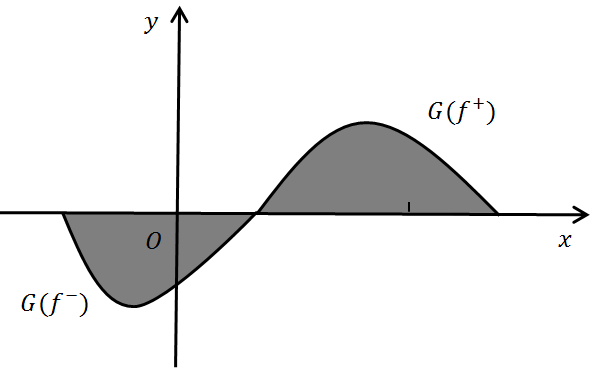
\includegraphics[width=0.6\textwidth]{image/Ljifenjiheyiyi.png}
\vspace*{-0.2cm}
\caption{~L-积分的几何意义} \label{fig41} 
\end{figure}


\section{勒贝格积分的性质}

\subsection{L-积分的基本性质}

\begin{proposition} \label{prop413}
设~$f(x),\, g(x)$~在~$E$~上的~L-积分存在, 则

(i) 对~$\forall~c \in \mathbb{R}$, $c f(x)$~的~L-积分存在, 且~$\int_E c f(x) \d \mu = c \int_E f(x) \d \mu$;

(ii) 若~$\int_E f(x) \d \mu + \int_E g(x) \d \mu$~有意义, 则~$f(x) + g(x)$~的~L-积分存在, 且
\[
\int_E \big[f(x) + g(x)\big] \d \mu = \int_E f(x) \d \mu + \int_E g(x) \d \mu
\]

(iii) 若~$f(x) \leqslant g(x),\,  \mathrm{~a.e.~} x \in E$, 则~$\int_E f(x) \d \mu \leqslant \int_E g(x) \d \mu$.
\end{proposition}

\begin{proof}
(i) 若~$c \geqslant 0$, 则~$(cf)^+ = c f^+,\, (cf)^- = c f^-$. 由~$f$~的~L-积分存在易知~$cf$~的~L-积分也存在. 再由命题~\ref{prop412}
\begin{eqnarray*}
\int_E cf(x) \d \mu &=& \int_E (cf)^+(x) \d \mu - \int_E (cf)^-(x) \d \mu \\
&=& \int_E c f^+(x) \d \mu - \int_E c f^-(x) \d \mu \\
&=& c \int_E f(x) \d \mu
\end{eqnarray*}
若~$c < 0$, 则~$(cf)^+ = -c f^-, \, (cf)^- = -c f^+$. 类似可证结论成立.

(ii) 由于~$(f+g)^+ - (f+g)^- = f + g = f^+ - f^- + g^+ - g^-$, 故
\[
(f+g)^+ + f^- + g^- = (f+g)^- + f^+ + g^+
\]
两边同时积分, 再由命题~\ref{prop412}, 得
\begin{eqnarray} \label{eq41}
&& \int_E (f+g)^+(x) \d \mu + \int_E f^-(x) \d \mu + \int_E g^-(x) \d \mu \nonumber \\
&=& \int_E (f+g)^-(x) \d \mu + \int_E f^+(x) \d \mu + \int_E g^+(x) \d \mu
\end{eqnarray}
注意到
\[
(f+g)^+ \leqslant f^+ + g^+,  \quad  (f+g)^- \leqslant f^- + g^-
\]
则有
\[
\int_E (f+g)^+(x) \d \mu \leqslant \int_E f^+(x) \d \mu + \int_E g^+(x) \d \mu
\]
\[
\int_E (f+g)^-(x) \d \mu \leqslant \int_E f^-(x) \d \mu + \int_E g^-(x) \d \mu
\]
由于~$\int_E f(x) \d \mu + \int_E g(x) \d \mu$~有意义, 故~$\int_E f^+(x) + \int_E g^+(x)$~与~$\int_E f^-(x) + \int_E g^-(x)$~至少有一个是有限的.

不妨设~$\int_E f^-(x) + \int_E g^-(x) < +\infty$, 从而~$\int_E (f+g)^-(x) \d \mu < +\infty$. 用式~\eqref{eq41}~两端同时减去
\[
\int_E (f+g)^-(x) \d \mu + \int_E f^-(x) \d \mu + \int_E g^-(x) \d \mu
\]
得
\begin{eqnarray*}
&& \int_E (f+g)^+(x) \d \mu - \int_E (f+g)^-(x) \d \mu \\
&=& \int_E f^+(x) \d \mu + \int_E g^+(x) \d \mu - \int_E f^-(x) \d \mu - \int_E g^-(x) \d \mu
\end{eqnarray*}
即
\[
\int_E \big[f(x) + g(x)\big] \d \mu = \int_E f(x) \d \mu + \int_E g(x) \d \mu
\]
这也表明~$f(x) + g(x)$~的~L-积分存在.

(iii) $f(x) \leqslant g(x),\, \mathrm{~a.e.~} x \in E$, 则~$f^+(x) \leqslant g^+(x),\, \mathrm{~a.e.~} x \in E$, $f^-(x) \geqslant g^-(x),\, \mathrm{~a.e.~} x \in E$. 由命题~\ref{prop412}~(iii)
\[
\int_E f^+(x) \d \mu \leqslant \int_E g^+(x) \d \mu, \quad \int_E f^-(x) \d \mu \geqslant \int_E g^-(x) \d \mu
\]
从而
\begin{eqnarray*}
\int_E f(x) \d \mu &=& \int_E f^+(x) \d \mu - \int_E f^-(x) \d \mu \\
&\leqslant& \int_E g^+(x) \d \mu - \int_E g^-(x) \d \mu = \int_E g(x) \d \mu
\end{eqnarray*}
故结论成立.
\end{proof}

\begin{remark}
特别地, ``~L-积分存在''换成~``~L-可积'', 相应的结论也成立.
\end{remark}

\begin{theorem} \label{thm421}
若~$f(x) = g(x),\, \mathrm{~a.e.~} x \in E$, 则~$\int_E f(x) \d \mu = \int_E g(x) \d \mu$.
\end{theorem}

\begin{proof}
由于~$f(x) = g(x)~\Leftrightarrow~f(x) \geqslant g(x)$~且~$f(x) \leqslant g(x)$,  再由命题~\ref{prop413}~(iii)~可得.
\end{proof}

定理~\ref{thm421}~表明, 函数改变零测集上的取值, 不影响其~L-积分值.

\begin{corollary}
(i) 若~$f(x) = 0,\, \mathrm{~a.e.~} x \in E$, 则~$\int_E f(x) \d \mu = 0$;

(ii) 若~$m(E) = 0$, 则对任意~$E$~上的可测函数~$f(x)$, 都有~$\int_E f(x) \d \mu = 0$;
\end{corollary}

\begin{proposition}
若~$f(x)$~在~$E$~上的~L-积分存在, 则~$\big| \int_E f(x) \d \mu \big| \leqslant \int_E |f(x)| \d \mu$.
\end{proposition}

\begin{proof}
$f$~的~L-积分存在, 则~$|f|$~的~L-积分也存在. 由于
\[
-|f(x)| \leqslant f(x) \leqslant |f(x)|
\]
由命题~\ref{prop413}~知
\[
-\int_E |f(x)| \d \mu \leqslant \int_E f(x) \d \mu \leqslant \int_E |f(x)| \d \mu
\]
故~$\big| \int_E f(x) \d \mu \big| \leqslant \int_E |f(x)| \d \mu$.
\end{proof}

\begin{theorem} \label{thm422}
$f(x)$~在~$E$~上~L-可积~$\Leftrightarrow$~$|f(x)|$~在~$E$~上~L-可积.
\end{theorem}

\begin{proof}
``$\Rightarrow$''. $f(x)$~在~$E$~上~L-可积, 则
\[
\int_E f^+(x) \d \mu < +\infty, \, \int_E f^-(x) \d \mu < +\infty
\]
又
\[
|f(x)| = f^+(x) + f^-(x)
\]
故
\[
0 < \int_E |f(x)| \d \mu = \int_E f^+(x) \d \mu + \int_E f^-(x) \d \mu < +\infty
\]
因此, $|f(x)|$~在~$E$~上~L-可积.

``$\Leftarrow$''. $|f(x)|$~在~$E$~上~L-可积, 则~$\int_E |f(x)| \d \mu < +\infty$. 故
\[
\Big|\int_E f(x) \d \mu \Big| \leqslant \int_E |f(x)| \d \mu < +\infty
\]
因此, $f(x)$~在~$E$~上~L-可积.
\end{proof}

\begin{theorem}
设~$m(E) < +\infty,\,  f(x)$~为~$E$~上的有界可测函数, 则~$f(x)$~在~$E$~上~L-可积.
\end{theorem}

\begin{proof}
$f(x)$~在~$E$~上有界, 则存在~$M > 0$~使得
\[
|f(x)| \leqslant M, \quad  \forall~x \in E
\]
从而
\[
\int_E |f(x)| \d \mu \leqslant \int_E M \d \mu = M \cdot m(E) < +\infty
\]
故~$|f(x)|$~在~$E$~上~L-可积, 再由定理~\ref{thm422}, $f(x)$~在~$E$~上~L-可积.
\end{proof}

\begin{proposition}
设~$f(x)$~在~$E$~上的~L-积分存在, 则

(i) $f(x)$~在~$E$~的任意可测子集~$E_0$~上的~L-积分也存在;

(ii) 设~$E_1,\, E_2$~为~$E$~的可测子集, 且~$E_1 \smallcap E_2 = \emptyset$, 则
\[
\int_{E_1 \cup E_2} f(x) \d \mu = \int_{E_1} f(x) \d \mu + \int_{E_2} f(x) \d \mu
\]
\end{proposition}

\begin{proof}
(i) 对任意可测集~$E_0 \subset E$, 都有
\[
\int_{E_0} f^+(x) \d \mu \leqslant \int_E f^+(x) \d \mu,
\quad \int_{E_0} f^-(x) \d \mu \leqslant \int_E f^-(x) \d \mu
\]
又~$f$~在~$E$~上的~L-积分存在, 则~$\int_E f^+(x) \d \mu$~与~$\int_E f^-(x) \d \mu$~至少有一个有限. 从而~$\int_{E_0} f^+(x) \d \mu$~与~$\int_{E_0} f^-(x) \d \mu$~至少有一个有限,  故~$f(x)$~在~$E_0$~上的~L-积分存在.

(ii) 由~(i)~知~(ii)~中的~L-积分都存在, $E_1 \smallcap E_2 = \emptyset$, 则
\[
\chi_{E_1 \cup E_2}(x) = \chi_{E_1}(x) + \chi_{E_2}(x)
\]
从而
\begin{eqnarray*}
\int_{E_1 \cup E_2} f(x) \d \mu &=& \int_{\mathbb{R}^n} f(x) \chi_{E_1 \cup E_2}(x) \d \mu \\
&=& \int_{\mathbb{R}^n} f(x) \big[\chi_{E_1}(x) + \chi_{E_2}(x) \big] \d \mu \\
&=& \int_{\mathbb{R}^n} f(x) \chi_{E_1}(x) \d \mu + \int_{\mathbb{R}^n} f(x) \chi_{E_2}(x) \d \mu \\
&=& \int_{E_1} f(x) \d \mu + \int_{E_2} f(x) \d \mu
\end{eqnarray*}
故结论成立.
\end{proof}

\begin{remark}
``L-积分存在''换成``L-可积'', 相应结论也成立. (ii)~的结论推广到有限个集合仍成立.
\end{remark}

\begin{theorem}
设~$f(x)$~在~$E$~上~L-可积, 则~$f(x)$~在~$E$~上几乎处处有限.
\end{theorem}

\begin{proof}
记~$E_\infty = \{x \in E: \: |f(x)| = +\infty\}$, 下面证明~$m(E_\infty) = 0$. 令
\[
E_n = \{x \in E: \: |f(x)| \geqslant n\}
\]
则~$\{E_n\}$~是单调递减的可测集列, 且~$E_\infty = \mathop{\smallcap}\limits_{n=1}^\infty E_n$. 又~$f(x)$~在~$E$~上~L-可积, 则~$|f(x)|$~~在~$E$~上~L-可积, 从而对每个~$n \in \mathbb{N}$, 都有
\[
n \cdot m(E_n) \leqslant \int_{E_n} |f(x)| \d \mu < \int_E |f(x)| \d \mu < +\infty
\]
故~$m(E_n) \to 0,\, n \to \infty$. 从而由单调可测集列测度的极限性质
\[
m(E_\infty) = m\Big( \medcap_{n=1}^\infty E_n \Big) = \lim_{n \to \infty} m(E_n) = 0
\]
因此, $f(x)$~在~$E$~上几乎处处有限.
\end{proof}

\begin{theorem} \label{thm425}
设~$f(x)$~为~$E$~上可测函数, 且~$\int_E |f(x)| \d \mu = 0$, 则~$f(x) = 0, \, \mathrm{~a.e.~} x \in E$.
\end{theorem}

\begin{proof}
记~$E_0 = \{x \in E: \: |f(x)| > 0\}$, 下面证明~$m(E_0) = 0$. 由于~$f$~可测, 则~$|f|$~可测. 令
\[
E_n = \Big\{x \in E: \: |f(x)| \geqslant \frac{1}{n}\Big\}
\]
则~$\{E_n\}$~是单调递增的可测集列, 且~$E_0 = \mathop{\cup}\limits_{n=1}^\infty E_n$. 由单调可测集列测度的极限性质
\[
m(E_0) = m\big(\medcup_{n=1}^\infty E_n\big) = \lim_{n \to \infty} m(E_n)
\]
若~$m(E_0) > 0$, 则对~$m(E_0)/2$, 存在~$n_0 \in \mathbb{N}$~使得
\[
m\big(E_{n_0}\big) > m(E_0)/2
\]
注意到, 当~$x \in E_{n_0}$~时, 有~$|f(x)| \geqslant 1/n_0$. 从而
\begin{eqnarray*}
\int_E |f(x)| \d \mu &=& \int_{E_0} |f(x)| \d \mu \geqslant \int_{E_{n_0}} |f(x)| \d \mu \\
&\geqslant& \int_{E_{n_0}} \frac{1}{n_0} \d \mu = \frac{1}{n_0} \cdot m\big(E_{n_0}\big) \\
&>& \frac{m(E_0)}{2n_0} > 0
\end{eqnarray*}
矛盾, 故~$m(E_0) = 0$. 因此, $f(x) = 0, \, \mathrm{~a.e.~} x \in E$.
\end{proof}

\begin{theorem}[L-积分的绝对连续性\index{勒贝格积分的绝对连续性}]
设~$f(x)$~在~$E$~上~L-可积, 则对~$\forall~\varepsilon > 0$, 都存在~$\delta > 0$, 使得当~$e \subset E, \, m(e) < \delta$~时, 有
\[
\Big| \int_e f(x) \d \mu \Big| \leqslant \int_e |f(x)| \d \mu < \varepsilon
\]
\end{theorem}

\begin{proof}
$f$~在~$E$~上~L-可积, 则~$|f|$~在~$E$~上~L-可积. 又~$|f(x)|$~是非负可测函数, 由定理~\ref{thm411},  存在非负简单函数列~$\{\varphi_n\} \nearrow |f|$, 且
\[
\lim_{n \to \infty} \int_E \varphi_n(x) \d \mu = \int_E |f(x)| \d \mu < +\infty
\]
故对~$\forall~\varepsilon > 0$, 存在~$n_0 \in \mathbb{N}$~使得
\[
0 \leqslant \int_E \big[ |f(x)| - \varphi_{n_0}(x) \big] \d \mu < \frac{\varepsilon}{2}
\]
又简单函数是有界函数, 故存在~$M > 0$~使得
\[
0 \leqslant \varphi_{n_0}(x) \leqslant M, \quad  \forall~x \in E
\]
令~$\delta = \varepsilon/2M$, 则对任意的~$e \subset E, \, m(e) < \delta$, 有
\begin{eqnarray*}
\int_e |f(x)| \d \mu &=& \int_e \big[ |f(x)| - \varphi_{n_0}(x) \big] \d \mu + \int_e \varphi_{n_0}(x) \d \mu \\
&\leqslant& \int_E \big[ |f(x)| - \varphi_{n_0}(x) \big] \d \mu + \int_e M \d \mu \\
&<& \frac{\varepsilon}{2} + M \cdot m(e) \\
&<& \frac{\varepsilon}{2} + \frac{\varepsilon}{2} = \varepsilon
\end{eqnarray*}
定理得证.
\end{proof}

勒贝格积分的绝对连续性表明, 当积分区域很小(趋于~$0$)时, 积分值也很小(趋于~$0$).

\begin{theorem}[积分变量的平移变换] \label{thm427}
设~$f(x)$~在~$\mathbb{R}^n$~上~L-可积, 则对~$\forall~h \in \mathbb{R}^n$,   都有~$f(x + h)$~也在~$\mathbb{R}^n$~上~L-可积, 且
\[
\int_{\mathbb{R}^n} f(x + h) \d \mu = \int_{\mathbb{R}^n} f(x) \d \mu
\]
\end{theorem}

\begin{proof}
只需考虑非负可测函数情形.

(i) 若~$f(x)$~是非负简单函数, 记
\[
f(x) = \sum_{k=1}^m c_k \chi_{E_k}(x), \quad x \in \mathbb{R}^n
\]
其中, $\{E_k\}$~可测、互不相交, 且~$\mathop{\smallcup}\limits_{k=1}^m = \mathbb{R}^n$. 显然
\[
f(x+h) = \sum_{k=1}^m c_k \chi_{E_k - \{h\}}(x), \quad x \in \mathbb{R}^n
\]
也是非负简单函数, 从而由测度的平移不变性
\[
\int_{\mathbb{R}^n} f(x + h) \d \mu = \sum_{k=1}^m c_k m\big( E_k - \{h\} \big)
= \sum_{k=1}^m c_k m(E_k) = \int_{\mathbb{R}^n} f(x) \d \mu
\]

(ii) 若~$f(x)$~是一般的非负可测函数, 则存在递增的非负简单函数列~$\{\varphi_n(x)\}$, 使得
\[
\lim_{n \to \infty} \varphi_n(x) = f(x), \quad x \in \mathbb{R}^n
\]
显然, $\{\varphi_n(x + h)\}$~仍是递增的非负简单函数列, 且
\[
\lim_{n \to \infty} \varphi_n(x+h) = f(x+h), \quad x \in \mathbb{R}^n
\]
从而, 由定理~\ref{thm411}~及~(i)
\begin{eqnarray*}
\int_{\mathbb{R}^n} f(x + h) \d \mu &=& \int_{\mathbb{R}^n} \lim_{n \to \infty} \varphi_n(x+h) \d \mu = \lim_{n \to \infty} \int_{\mathbb{R}^n} \varphi_n(x+h) \d \mu \\
&=& \lim_{n \to \infty} \int_{\mathbb{R}^n} \varphi_n(x) \d \mu =  \int_{\mathbb{R}^n} \lim_{n \to \infty} \varphi_n(x) \d \mu \\
&=& \int_{\mathbb{R}^n} f(x) \d \mu
\end{eqnarray*}
定理得证.
\end{proof}

\subsection{L-可积函数与连续函数}

下面讨论~L-可积函数与连续函数的关系: L-可积函数可用连续函数平均逼近.

\begin{lemma} \label{lem432}
设~$f(x)$~在~$E$~上~L-可积, 则对~$\forall~ \varepsilon > 0$, 都存在~$E$~上的简单函数~$\varphi(x)$~使得
\[
\int_E \big|f(x) - \varphi(x) \big| \d \mu < \varepsilon
\]
此时称~$f(x)$~可由~$\varphi(x)$~平均逼近\index{平均逼近}.
\end{lemma}

\begin{proof}
记~$f(x) = f^+(x) - f^-(x)$, 由非负可测函数~L-积分的定义知, 对~$\forall~ \varepsilon > 0$,  存在非负简单函数~$\varphi^+ \leqslant f^+, \, \varphi^- \leqslant f^-$~使得
\[
\int_E f^+(x) \d \mu - \int_E \varphi^+(x) \d \mu < \frac{\varepsilon}{2}
\]
\[
\int_E f^-(x) \d \mu - \int_E \varphi^-(x) \d \mu < \frac{\varepsilon}{2}
\]
令~$\varphi = \varphi^+ - \varphi^-$, 则~$\varphi(x)$~是~$E$~上的简单函数, 且
\begin{eqnarray*}
\int_E \big|f(x) - \varphi(x) \big| \d \mu &\leqslant& \int_E \big|f^+(x) - \varphi^+(x) \big| \d \mu + \int_E \big|f^-(x) - \varphi^-(x) \big| \d \mu \\
&=& \int_E \big[f^+(x) - \varphi^+(x) \big] \d \mu + \int_E \big[f^-(x) - \varphi^-(x) \big] \d \mu \\
&<& \frac{\varepsilon}{2} + \frac{\varepsilon}{2} = \varepsilon
\end{eqnarray*}
引理得证.
\end{proof}

\begin{theorem}
设~$f(x)$~为~$E$~上的~L-可积函数, 则对~$\forall~ \varepsilon > 0$,  都存在~$\mathbb{R}^n$~上具有紧支集的连续函数~$g(x)$~使得
\[
\int_E \big|f(x) - g(x) \big| \d \mu < \varepsilon
\]
\end{theorem}

\begin{proof}
$f(x)$~为~$E$~上的~L-可积函数, 由引理~\ref{lem432}, 对~$\forall~ \varepsilon > 0$,  存在~$E$~上的简单函数~$\varphi(x)$~使得
\[
\int_E \big|f(x) - \varphi(x) \big| \d \mu < \frac{\varepsilon}{2}
\]
又简单函数是有界函数, 不妨设~$|\varphi(x)| \leqslant M$. 由定理~\ref{thm333}, 对上述的~$\varepsilon$,  存在~$\mathbb{R}^n$~上具有紧支集的连续函数~$g(x)$~满足~$|g(x)| \leqslant M,  \,  \forall~x \in \mathbb{R}^n$, 且
\[
m\big( \{x \in E: \: |\varphi(x) - g(x)| > 0\} \big) < \frac{\varepsilon}{4M}
\]
从而
\begin{eqnarray*}
\int_E \big|\varphi(x) - g(x)\big| \d \mu &=& \int\limits_{E_{[|\varphi - g|> 0]}} \big|\varphi(x) - g(x)\big| \d \mu \\
&\leqslant& 2 M \cdot m\big( \{x \in E: \: |\varphi(x) - g(x)| > 0\} \big) \\
&<& \frac{\varepsilon}{2}
\end{eqnarray*}
因此
\begin{eqnarray*}
\int_E \big|f(x) - g(x)\big| \d \mu &\leqslant& \int_E \big|f(x) - \varphi(x)\big| \d \mu + \int_E \big|\varphi(x) - g(x)\big| \d \mu \\
&<& \frac{\varepsilon}{2} + \frac{\varepsilon}{2} = \varepsilon
\end{eqnarray*}
定理得证.
\end{proof}

\begin{remark}
该定理表明, 若~$f(x)$~在~$E$~上~L-可积, 则存在~$f$~的分解
\[
f(x) = g(x) + [f(x) - g(x)] = f_1(x) + f_2(x),  \quad x \in E
\]
其中, $f_1(x)$~为~$\mathbb{R}^n$~上具有紧支集的连续函数, $|f_2(x)|$~在~$E$~上的~L-积分任意小.
\end{remark}

\begin{theorem}[平均连续性\index{平均连续性}]
设~$f(x)$~为~$\mathbb{R}^n$~上的~L-可积函数, 则
\[
\lim_{h \to 0} \int_{\mathbb{R}^n} \big| f(x + h) - f(x) \big| \d \mu = 0
\]
\end{theorem}

\begin{proof}
对~$\forall~ \varepsilon > 0$, 作分解~$f(x) = f_1(x) + f_2(x)$, 其中, $f_1(x)$~为~$\mathbb{R}^n$~上具有紧支集的连续函数, $f_2(x)$~满足
\[
\int_{\mathbb{R}^n} \big|f_2(x)\big| \d \mu < \frac{\varepsilon}{4}
\]
由于紧集上的连续函数是一致连续的, 故易知对上述的~$\varepsilon$, 存在~$\delta > 0$, 使得当~$|h| < \delta$~时有
\[
\int_{\mathbb{R}^n} \big|f_1(x + h) - f_1(x) \big| \d \mu < \frac{\varepsilon}{2}
\]
从而, 由定理~\ref{thm427}
\begin{eqnarray*}
&& \int_{\mathbb{R}^n} \big| f(x + h) - f(x) \big| \d \mu \\
&\leqslant& \int_{\mathbb{R}^n} \big| f_1(x + h) - f_1(x) \big| \d \mu + \int_{\mathbb{R}^n} \big| f_2(x + h) - f_2(x) \big| \d \mu \\
&<& \frac{\varepsilon}{2} + \int_{\mathbb{R}^n} \big| f_2(x + h) \big| \d \mu + \int_{\mathbb{R}^n} \big| f_2(x) \big| \d \mu \\
&=& \frac{\varepsilon}{2} + 2 \int_{\mathbb{R}^n} \big| f_2(x) \big| \d \mu \\
&<& \varepsilon
\end{eqnarray*}
定理得证.
\end{proof}

\section{勒贝格积分的极限定理}

勒贝格积分的极限定理有三个重要定理, 即列维定理(单调收敛定理), 法都引理和勒贝格控制收敛定理.

\subsection{列维定理}

\begin{lemma} \label{lem431}
设~$\{E_n\}$~为单调的可测集列, $\varphi(x)$~为非负简单函数, 则
\[
\lim_{n \to \infty}  \int_{E_n} \varphi(x) \d \mu = \int_{\lim\limits_{n \to \infty} E_n} \varphi(x) \d \mu
\]
\end{lemma}

\begin{proof}
设~$\{E_n\}$~单调递增, 则~$\lim\limits_{n \to \infty} E_n = \mathop{\smallcup}\limits_{n=1}^\infty E_n$,  记为~$E$.

记~$\varphi(x) = \sum\limits_{k=1}^m a_k \chi_{A_k} (x)$, 注意到~$\{E_n \smallcap A_k\}_{n=1}^\infty$~是单调递增可测集列, 由单调集列测度的极限性质可得
\begin{eqnarray*}
\lim_{n \to \infty} \int_{E_n} \varphi(x) \d \mu &=& \lim_{n \to \infty} \sum_{k=1}^m a_k m(E_n \medcap A_k) \\
&=& \sum_{k=1}^m \lim_{n \to \infty} a_k m(E_n \medcap A_k) = \sum_{k=1}^m a_k m\Big(\medcup_{n=1}^\infty (E_n \medcap A_k)\Big) \\
&=& \sum_{k=1}^m a_k m(E \medcap A_k) = \int_E \varphi(x) \d \mu
\end{eqnarray*}
类似可证, 对于单调递减集列结论也成立.
\end{proof}

\begin{theorem}[列维定理\index{列维定理}]
设~$\{f_n(x)\}$~为~$E$~上的非负可测函数, 满足
\[
f_1(x) \leqslant \cdots \leqslant f_n(x) \leqslant \cdots \quad \mathrm{~a.e.~} x \in E
\]
且~$f_n \xrightarrow{\mathrm{a.e.}} f$, 即~$\lim\limits_{n \to \infty} f_n(x) = f(x),\, \mathrm{~a.e.~} x \in E$. 则
\[
\lim_{n \to \infty} \int_E f_n(x) \d \mu = \int_E f(x) \d \mu
\]
\end{theorem}

\begin{proof}
由~L-积分的单调性, 有
\[
\int_E f_1(x) \d \mu \leqslant \cdots \leqslant \int_E f_n(x) \d \mu \leqslant \cdots \leqslant \int_E f(x) \d \mu
\]
故~$\lim\limits_{n \to \infty} \int_E f_n(x) \d \mu$~存在(或~$=+\infty$), 且
\[
\lim_{n \to \infty} \int_E f_n(x) \d \mu \leqslant \int_E f(x) \d \mu
\]
下面证明相反的不等式.

任取~$c \in (0,\, 1)$, 以及非负简单函数~$\varphi(x)$~满足~$\varphi \leqslant f$. 记
\[
E_n = \{x \in E: \: f_n(x) \geqslant c ~\! \varphi(x)\}, \quad  n = 1,\, 2,\, \cdots
\]
则~$\{E_n\}$~是单调递增的可测集列, 且~$\lim\limits_{n \to \infty} E_n = E$.

事实上, 只需验证~$E \subset \mathop{\smallcup}\limits_{n=1}^\infty E_n$. 对~$\forall~x \in E$, 都有~$f(x) \geqslant \varphi(x)$. 由于
\[
\lim_{n \to \infty} f_n(x) = f(x) \geqslant \varphi(x)
\]
则对上述的~$c$, 存在~$n_0 \in \mathbb{N}$~使得
\[
f_{n_0}(x) > c ~\! f(x) \geqslant c ~\! \varphi(x)
\]
故~$x \in E_{n_0} \subset \mathop{\smallcup}\limits_{n=1}^\infty E_{n}$, 从而~$E \subset \mathop{\smallcup}\limits_{n=1}^\infty E_{n}$.

\vspace*{0.2cm}

于是, 由引理~\ref{lem431}~可得
\[
\lim_{n \to \infty} \int_{E_n} \varphi(x) \d \mu = \int_E \varphi(x) \d \mu
\]
从而
\begin{eqnarray*}
\lim_{n \to \infty} \int_E f_n(x) \d \mu &\geqslant& \lim_{n \to \infty} \int_{E_n} f_n(x) \d \mu \\
&\geqslant& \lim_{n \to \infty} \int_{E_n} c ~\! \varphi(x) \d \mu = c ~\! \int_E \varphi(x) \d \mu
\end{eqnarray*}
令~$c \to 1$~得~$\lim\limits_{n \to \infty} \int_E f_n(x) \d \mu \geqslant \int_E \varphi(x) \d \mu$. 再由~$\varphi(x)$~的任意性, 以及~$\int_E f(x) \d \mu$~的定义可得
\[
\lim_{n \to \infty} \int_E f_n(x) \d \mu \geqslant \int_E f(x) \d \mu
\]
定理得证.
\end{proof}

\begin{remark}
(i) 该定理表明对于非负递增可测函数列, L-积分号与极限号是可交换的, 即
\[
\int_E \lim_{n \to \infty} f_n(x) \d \mu = \lim_{n \to \infty} \int_E f_n(x) \d \mu
\]

(ii) 列维定理的非负条件可以放宽到: ``存在~$E$上的~L-可积函数~$g$~使得, $f_n \geq g$''. 实际上，取~$F_n=f_n-g$, 再对~$\{F_n\}$~应用列维定理即可.
\end{remark}

\begin{theorem}[勒贝格逐项积分定理\index{勒贝格逐项积分定理}, 列维定理的级数形式]
设~$\{f_n(x)\}$~为~$E$~上的非负可测函数列, 则
\[
\int_E \sum_{n=1}^\infty f_n(x) \d \mu = \sum_{n=1}^\infty \int_E f_n(x) \d \mu
\]
\end{theorem}

\begin{proof}
令~$g_n(x) = \sum\limits_{k=1}^n f_k(x),\, n = 1,\,  2,\, \cdots$, 则~$g_n(x)$~非负可测, 单调递增收敛到~$\sum\limits_{n=1}^\infty f_n(x)$. 由列维定理
\begin{eqnarray*}
\int_E \sum_{n=1}^\infty f_n(x) \d \mu &=& \int_E \lim_{n \to \infty} \sum_{k=1}^n f_k(x) \d \mu = \int_E \lim_{n \to \infty} g_n(x) \d \mu \\
&=& \lim_{n \to \infty} \int_E g_n(x) \d \mu = \lim_{n \to \infty} \int_E \sum\limits_{k=1}^n f_k(x) \d \mu \\
&=& \lim_{n \to \infty} \sum\limits_{k=1}^n \int_E  f_k(x) \d \mu \\
&=& \sum_{n=1}^\infty \int_E f_n(x) \d \mu
\end{eqnarray*}
定理得证.
\end{proof}

\begin{proposition}[L-积分对积分区域的可数可加性\index{勒贝格积分区域的可数可加性}]
设~$\{E_n\}$~为互不相交的可测集列, $f(x)$~是~$\mathop{\smallcup}\limits_{n=1}^\infty E_n$~上的非负可测函数, 则
\[
\int_{\mathop{\medcup}\limits_{n=1}^\infty E_n} f(x) \d \mu = \sum_{n=1}^\infty \int_{E_n} f(x) \d \mu
\]
\end{proposition}

\begin{proof}
由逐项积分定理
\begin{eqnarray*}
\int_{\mathop{\medcup}\limits_{n=1}^\infty E_n} f(x) \d \mu &=& \int_{\mathbb{R}^n} f(x) \chi_{\mathop{\medcup}\limits_{n=1}^\infty E_n}(x) \d \mu = \int_{\mathbb{R}^n} f(x) \sum_{n=1}^\infty \chi_{E_n}(x) \d \mu \\
&=& \sum_{n=1}^\infty \int_{\mathbb{R}^n} f(x) \chi_{E_n}(x) \d \mu = \sum_{n=1}^\infty \int_{E_n} f(x) \d \mu
\end{eqnarray*}
命题得证.
\end{proof}

\begin{remark}
特别地, 当~$f(x) \equiv 1$~时, 上述结论恰好体现了测度的可数可加性. 可见通过点集的特征函数,
L-积分与测度问题是可以相互转化的.
\end{remark}

\begin{example}
设~$E_1,\, \cdots,\, E_n$~为~$[0,\, 1]$~中的可测集, 若~$[0,\, 1]$~中的每一点都至少属于其中
的~$k$~个($k \leqslant n$), 则必存在~$i_0$~使得~$m(E_{i_0}) \geqslant k/n$.
\end{example}

\begin{proof}
由题设当~$x \in [0,\, 1]$~时, 有~$\sum\limits_{i=1}^n \chi_{E_i}(x) \geqslant k$. 故
\begin{eqnarray*}
\sum_{i=1}^n m(E_i) &=& \sum_{i=1}^n \int_{[0,1]} \chi_{E_i}(x) \d \mu \\
&=& \int_{[0,1]} \sum_{i=1}^n \chi_{E_i}(x) \d \mu \geqslant \int_{[0,1]} k ~\! \d \mu = k
\end{eqnarray*}
若对每一个~$i$~都有~$m(E_i) < k/n$, 则
\[
\sum\limits_{i=1}^n m(E_i) < n \cdot \frac{k}{n} = k
\]
矛盾. 故存在~$i_0$~使得~$m(E_{i_0}) \geqslant k/n$.
\end{proof}

\begin{example}
设~$f(x)$~在~$[a,\, b]$~上~L-可积, 若
\[
\int_a^c f(x) \d \mu = 0, \quad  \forall~c \in [a,\, b]
\]
则~$f(x) = 0,\, \mathrm{~a.e.~} x \in [a,\, b]$.
\end{example}

\begin{proof}
假设~$f(x)$~在~$[a,\, b]$~上不几乎处处为~$0$, 不妨设~$E_0 = \{x \in [a,\, b]:\: f(x) > 0\}$, $m(E_0) > 0$,  则有
\[
\int_{E_0} f(x) \d \mu > 0
\]
由~L-积分的绝对连续性, 取
\[
\varepsilon = \frac{1}{2}\int_{E_0} f(x) \d \mu > 0
\]
存在~$\delta > 0$, 当~$m(e) < \delta$~时, 有
\[
\Big| \int_e f(x) \d \mu \Big| < \varepsilon = \frac{1}{2}\int_{E_0} f(x) \d \mu
\]
由于对~$\forall~[c,\, d] \subset [a,\, b]$, 都有
\[
\int_{(c, d)} f(x) \d \mu = \int_{(a, d)} f(x) \d \mu - \int_{(a,c)} f(x) \d \mu = 0
\]
则对任意开集~$G \subset [a,\, b]$, 由一维开集构造定理, $G = \mathop{\smallcup}_k (\alpha_k,\, \beta_k)$,  从而
\[
\int_G f(x) \d \mu = \sum_k \int_{(\alpha_k,\beta_k)} f(x) \d \mu = 0
\]
又~$E_0$~可测, 则存在开集~$G \supset E_0$, 使得~$m(G - E_0) < \delta$, 故
\[
\Big|\int_{G-E_0} f(x) \d \mu \Big| < \frac{1}{2}\int_{E_0} f(x) \d \mu
\]
于是
\begin{eqnarray*}
\int_G f(x) \d \mu &=& \int_{G-E_0} f(x) \d \mu + \int_{E_0} f(x) \d \mu \\
&\geqslant& \int_{E_0} f(x) \d \mu - \Big|\int_{G-E_0} f(x) \d \mu \Big| \\
&>& \frac{1}{2}\int_{E_0} f(x) \d \mu > 0
\end{eqnarray*}
矛盾.
\end{proof}

下面利用~L-积分对积分区域的可数可加性, 给出非负可测函数~L-可积的另一种等价描述:

\begin{theorem}
设~$m(E) < +\infty$, $f(x)$~为~$E$~上几乎处处有限的非负可测函数, 对值域~$[0,\,  +\infty)$~作划分
\[
0 = y_0 < y_1 < \cdots < y_n < y_{n+1} < \cdots \rightarrow +\infty
\]
其中, $y_{n+1} - y_n \leqslant \delta, \,, n = 0,\, 1,\, \cdots$. 记
\[
E_n = \{x \in E: \: y_n \leqslant f(x) < y_{n+1} \},  \quad n = 0,\, 1,\, \cdots
\]
则~$f(x)$~在~$E$~上~L-可积, 当且仅当~$\sum\limits_{n=0}^\infty y_n m(E_n) < +\infty$, 且
\[
\int_E f(x) \d \mu = \lim_{\delta \to 0} \sum_{n=0}^\infty y_n m(E_n)
\]
\end{theorem}

\begin{proof}
由于
\[
y_n m(E_n) \leqslant \int_{E_n} f(x) \d \mu \leqslant y_{n+1} m(E_n),  \quad n = 0,\, 1,\, \cdots
\]
故
\[
\sum_{n=0}^{\infty} y_n m(E_n) \leqslant \sum_{n=0}^{\infty} \int_{E_n} f(x) \d \mu \leqslant \sum_{n=0}^{\infty} y_{n+1} m(E_n)
\]
注意到~$\{E_n\}$~是互不相交的可测集列, 且~$\mathop{\smallcup}\limits_{n=0}^\infty E_n = E$, 由~L-积分对积分区域的可数可加性
\[
\mathop{\sum}\limits_{n=0}^{\infty} \int_{E_n} f(x) \d \mu = \int_E f(x) \d \mu
\]
从而
\begin{eqnarray*}
\sum_{n=0}^{\infty} y_n m(E_n) &\leqslant& \int_E f(x) \d \mu \leqslant \sum_{n=0}^{\infty} y_{n+1} m(E_n) \\
&=& \sum_{n=0}^{\infty} (y_{n+1}-y_n) m(E_n) + \sum_{n=0}^{\infty} y_n m(E_n) \\
&\leqslant& \delta m(E) + \sum_{n=0}^{\infty} y_n m(E_n)
\end{eqnarray*}
令~$\delta \to 0$~可得
\[
\int_E f(x) \d \mu = \lim_{\delta \to 0} \sum_{n=0}^\infty y_n m(E_n)
\]
\end{proof}

\subsection{法都引理}

\begin{theorem}[法都引理\index{法都引理}]
设~$\{f_n(x)\}$~为~$E$~上的非负可测函数列, 则
\[
\int_E \liminf_{n \to \infty} f_n(x) \d \mu \leqslant \liminf_{n \to \infty} \int_E f_n(x) \d \mu
\]
\end{theorem}

\begin{proof}
令~$u_k(x) = \inf\limits_{n \geq k} f_n(x),  \,  k = 1,\,  2,\, \cdots$,  则~$\{u_k(x)\}$~为递增的非负可测函数列, 且收敛到~$\liminf\limits_{n \to \infty} f_n(x)$, 故由列维定理得
\[
\int_E \liminf_{n \to \infty} f_n(x) \d \mu = \lim_{k \to \infty} \int_E u_k(x) \d \mu = \lim_{k \to \infty}  \int_E \inf_{n \geq k} f_n(x) \d \mu
\]
又~$\int_E \inf_{n \geq k} f_n(x) \d \mu \leqslant \int_E f_k(x) \d \mu$, 两边取~``$\liminf$'', 注意到左端极限存在，则有
\[
\lim_{k \to \infty}  \int_E \inf_{n \geq k} f_n(x) \d \mu \leqslant \liminf_{k \to \infty} \int_E f_k(x) \d \mu
\]
从而, $\int_E \liminf\limits_{n \to \infty} f_n(x) \d \mu \leqslant \liminf\limits_{n \to \infty} \int_E f_n(x) \d \mu$. 
\end{proof}

\begin{remark}
(i) 法都引理的非负条件可以放宽到: ``存在~$E$上的~L-可积函数~$g$~使得, $f_n \geq g$''. 

(ii) 法都引理中的~``$<$''~有可能成立. 例如, 考虑~$[0,\, 1]$~上的可测函数列~$\{f_n(x)\}$
\[
f_n(x) = \left\{\!\!
\begin{array}{ll}
n, & x \in \big(0,\, \frac{1}{n}\big) \\[0.2cm]
0, & x \in [0,\, 1] - \big(0,\, \frac{1}{n}\big)
\end{array}
\right.
\]
其中~$n = 1,\, 2,\, \cdots$, 则~$\lim\limits_{n \to \infty} f_n(x) = 0$. 故~$\int_E \liminf\limits_{n \to \infty} f_n(x) \d \mu = 0$. 而
\begin{eqnarray*}
\int_{[0,1]} f_n(x) \d \mu &=& n \cdot m\big(0,\, \frac{1}{n}\big) + 0 \cdot m\big( [0,\, 1] - (0,\, \frac{1}{n}) \big) \\
&=& n \cdot \frac{1}{n} + 0 \cdot \big( 1 - \frac{1}{n} \big) = 1
\end{eqnarray*}
于是~$\liminf\limits_{n \to \infty} \int_E f_n(x) \d \mu = 1$.
\end{remark}

\begin{remark}
列维定理~$\Leftrightarrow$~法都引理.
\end{remark}

\begin{proof}
法都引理就是利用列维定理得到的, 故只需证充分性. 设~$\{f_n(x)\}$~为~$E$~上的递增的非负可测函数列, 且满足~$\lim\limits_{n \to \infty} f_n(x) = f(x)$. 则~$\lim_{n \to \infty} \int_E f_n(x)  \d \mu$~存在，且由极限保号性有
\[
\lim_{n \to \infty} \int_E f_n(x)  \d \mu \leq \int_E f(x) \d \mu
\]
从而，由法都引理
\begin{eqnarray*}
\int_E f(x) \d \mu &=& \int_E \liminf_{n \to \infty} f_n(x) \d \mu \\
&\leqslant& \liminf_{n \to \infty} \int_E f_n(x) \d \mu = \lim_{n \to \infty} \int_E f_n(x) \d \mu
\end{eqnarray*}
故列维定理成立.
\end{proof}

\begin{corollary} \label{cor431}
设~$\{f_n\}$~为~$E$~上的可测函数列, 若存在~$E$~上的~L-可积函数~$h$, 使得~$f_n \leqslant h$, 则
\[
\int_E \limsup_{n \to \infty} f_n(x) \d \mu \geqslant \limsup_{n \to \infty} \int_E f_n(x) \d \mu
\]
\end{corollary}

\begin{proof}
对每个~$n \in \mathbb{N}$, 令~$g_n=-f_n$, 则~$g_n \geqslant -h$. 又~$-h$~在~$E$~上~L-可积，由法都引理的注知
\[
\int_E \liminf_{n \to \infty} g_n(x) \d \mu \leqslant \liminf_{n \to \infty} \int_E g_n(x) \d \mu
\]
即
\[
\int_E \liminf_{n \to \infty} (-f_n)(x) \d \mu \leqslant \liminf_{n \to \infty} \int_E (-f_n)(x) \d \mu
\]
注意到，$\inf (-A) = - \sup A$, 从而
\[
\int_E -\limsup_{n \to \infty} f_n(x) \d \mu \leqslant \liminf_{n \to \infty} \Big\{-\int_E f_n(x) \d \mu \Big\} = - \limsup_{n \to \infty} \int_E f_n(x) \d \mu
\]
于是
\[
\int_E \limsup_{n \to \infty} f_n(x) \d \mu \geqslant \limsup_{n \to \infty} \int_E f_n(x) \d \mu
\]
\end{proof}

\subsection{勒贝格控制收敛定理}

勒贝格控制收敛定理提供了~L-积分与极限可交换次序的一个充分条件, 这一结果是勒贝格积分理论最重要的结果之一, 在函数论、微分方程、概率论等学科有着相当广泛的应用.

\begin{theorem}[勒贝格控制收敛定理\index{勒贝格控制收敛定理}]
设~$\{f_n(x)\}$~为~$E$~上的可测函数列, 满足

(i) $f_n \xrightarrow{\mathrm{a.e.}} f$;

(ii) 存在非负~L-可积函数~$F(x)$~使得\footnote{~$F(x)$~通常称为函数列~$\{f_n(x)\}$~的控制函数. }
\[
|f_n(x)| \leqslant F(x),  \quad \mathrm{~a.e.~} x \in E,\quad  \forall~n \in \mathbb{N}
\]
则~$f(x)$~在~$E$~上~L-可积, 且
\[
\int_E f(x) \d \mu = \lim_{n \to \infty} \int_E f_n(x) \d \mu
\]
\end{theorem}

\begin{proof}
不妨设~$f_n \to f$. 由题设知, $-F \leq f_n \leq F$, 且~$-F, \, F$~在~$E$~上~L-可积，由法都引理的注和推论~\ref{cor431}~可得
\begin{eqnarray*}
\int_E f(x) \d \mu &=& \int_E \lim_{n \to \infty} f_n(x) \d \mu \\
&=& \int_E \liminf_{n \to \infty} f_n(x) \d \mu \leqslant \liminf_{n \to \infty} \int_E f_n(x) \d \mu \\
&\leqslant& \limsup_{n \to \infty} \int_E f_n(x) \d \mu \leqslant \int_E \limsup_{n \to \infty} f_n(x) \d \mu \\
&=& \int_E \lim_{n \to \infty} f_n(x) \d \mu = \int_E f(x) \d \mu
\end{eqnarray*}

故上式必须都取~``$=$''. 因此, $\int_E f(x) \d \mu = \lim\limits_{n \to \infty} \int_E f_n(x) \d \mu$.
\end{proof}

\begin{remark}
勒贝格控制收敛定理条件下, 积分号与极限号是可交换的, 即
\[
\int_E \lim_{n \to \infty} f_n(x) \d \mu = \lim_{n \to \infty} \int_E f_n(x) \d \mu
\]
\end{remark}

\begin{corollary}[有界收敛定理]
设~$m(E) < +\infty$, $\{f_n(x)\}$~为~$E$~上的一致有界可测函数列, 即存在~$M > 0$~使得
\[
|f_n(x)| \leqslant M,\quad  \forall~ x \in E,\,  \forall~n \in \mathbb{N}
\]
且满足~$f_n \xrightarrow{\mathrm{a.e.}} f$, 则~$f(x)$~在~$E$~上~L-可积, 且
\[
\int_E f(x) \d \mu = \lim_{n \to \infty} \int_E f_n(x) \d \mu
\]
\end{corollary}

\begin{proof}
取控制函数~$F(x) \equiv M$~即可.
\end{proof}

\begin{example}
求极限~${\displaystyle \lim\limits_{n \to \infty} \int_0^1 \frac{nx^\frac{1}{2}}{1+ n^2 x^2} \sin^5 nx ~\! \d x}$.
\end{example}

\begin{solution}
令
\[
f_n(x) = \frac{nx^\frac{1}{2}}{1+ n^2 x^2} \sin^5 nx,\quad  x \in [0,\, 1]
\]
则~$f(x)$~为~$[0,\, 1]$~上的可测函数, 且
\[
|f_n(x)| = \Big| \frac{nx^\frac{1}{2}}{1+ n^2 x^2} \sin^5 nx \Big| \leqslant \Big| \frac{nx^\frac{1}{2}}{1+ n^2 x^2} \Big| \leqslant \Big| \frac{nx^\frac{1}{2}}{2 n x} \Big| = \frac{1}{2\sqrt{x}}
\]
而~$1/(2\sqrt{x})$~在~$[0,\, 1]$~上~L-可积, 由勒贝格控制收敛定理
\[
\lim_{n \to \infty} \int_0^1 \frac{nx^\frac{1}{2}}{1+ n^2 x^2} \sin^5 nx ~\! \d x = \int_0^1 \lim_{n \to \infty} \frac{nx^\frac{1}{2}}{1+ n^2 x^2} \sin^5 nx ~\! \d x = 0
\]
\end{solution}

若~$m(E) < +\infty$, 勒贝格控制收敛定理的条件~``$f_n \xrightarrow{\mathrm{a.e.}} f$''~可以放宽到更一般的~``$f_n \xrightarrow{~\mu~} f$'', 从而可以得到更一般的控制收敛定理:

\begin{theorem}
设~$m(E) < +\infty$, $\{f_n(x)\}$~为~$E$~上的可测函数列, 满足~$f_n \xrightarrow{~\mu~} f$,  且存在非负~L-可积函数~$F(x)$~使得
\[
|f_n(x)| \leqslant F(x),  \quad \mathrm{~a.e.~} x \in E
\]
则~$f(x)$~在~$E$~上~L-可积, 且
\[
\int_E f(x) \d \mu = \lim_{n \to \infty} \int_E f_n(x) \d \mu
\]
\end{theorem}

\begin{proof}
由于~$f_n \xrightarrow{~\mu~} f$, 由里斯定理, 存在子列~$\{f_{n_k}\} \subset \{f_n\}$~使得~$f_{n_k} \xrightarrow{\mathrm{a.e.}} f$. 又
\[
|f_{n_k}(x)| \leqslant F(x),  \,  \mathrm{~a.e.~} x \in E, \,  \forall~k \in \mathbb{N}
\]
令~$k \to \infty$~得
\[
|f(x)| \leqslant F(x),  \quad \mathrm{~a.e.~} x \in E
\]
故由~$F(x)$~在~$E$~上~L-可积知, $f(x)$~在~$E$~上~L-可积.

$F(x)$~在~$E$~上~L-可积, 由~L-积分的绝对连续性, 对~$\forall~\varepsilon > 0$, $\exists~ \delta > 0$,  使得当~$e \subset E, \, m(e) < \delta$~时有
\[
\int_e F(x) \d \mu < \frac{\varepsilon}{4}
\]
取~$\eta > 0$~满足~$\eta \cdot m(E) < \varepsilon/2$. 由于~$f_n \xrightarrow{~\mu~} f$, 故
对上述的~$\delta$~及~$\eta$, 存在~$n_0 \in \mathbb{N}$, 使得当~$n \geqslant n_0$~时, 有
\[
m \big( \{x \in E: \: |f_n(x) - f(x)| \geqslant \eta\} \big) < \delta
\]
于是, 当~$n \geqslant n_0$~时, 有
\begin{eqnarray*}
&&\Big| \int_E f_n(x) \d \mu - \int_E f(x) \d \mu \Big| \leqslant \int_E \big| f_n(x) - f(x) \big| \d \mu \\[0.2cm]
&=& \int\limits_{E_{[|f_n- f| \geqslant \eta]}} \big| f_n(x) - f(x) \big| \d \mu + \int\limits_{E_{[|f_n - f| < \eta]}} \big| f_n(x) - f(x) \big| \d \mu \\[0.2cm]
&\leqslant& \int\limits_{E_{[|f_n- f| \geqslant \eta]}} 2 F(x) \d \mu + \eta \cdot m(E) \\[0.2cm]
&<& 2 \cdot \frac{\varepsilon}{4} + \frac{\varepsilon}{2} = \varepsilon
\end{eqnarray*}
因此, 定理结论成立.
\end{proof}

\section{勒贝格积分与黎曼积分}

前三节已经基本建立了勒贝格积分理论, 本节将揭示勒贝格积分与黎曼积分的关系, 这一关系将用一个公式来表达, 它不但说明了勒贝格积分是黎曼积分的一种推广, 而且为一般有界实值函数黎曼可积提供了一个简明的判别准则.


\subsection{黎曼积分\index{黎曼积分}回顾}

设~$f(x)$~为定义在~$[a,\, b]$~上的有界实值函数, 作~$[a,\, b]$~的分割
\[
\Delta = \{x_0,\, x_1,\, \cdots, \, x_n\}
\]
其中
\[
a = x_0 < x_1 < \cdots < x_n = b
\]
记
\[
\|\Delta\| = \max \{ |x_i - x_{i-1}|: \: 1 \leqslant i \leqslant n\}
\]
设~$\Delta_1,\, \Delta_2$~为~$[a,\, b]$~的两个分割, 若~$\Delta_1 \subset \Delta_2$, 则称~$\Delta_2$~是~$\Delta_1$~的加细.

\smallskip

对每个~$i = 1,\, \cdots,\, n$, 记
\[
m_i = \inf\{f(x): \: x_{i-1} \leqslant x \leqslant x_i\},  \,  \quad M_i = \sup\{f(x): \: x_{i-1} \leqslant x \leqslant x_i\}
\]
则~$f(x)$~关于分割~$\Delta$~的达布下和与达布上和分别定义为
\[
s(f,\, \Delta) = \sum_{i=1}^n m_i (x_i - x_{i-1}),  \quad S(f,\, \Delta) = \sum_{i=1}^n M_i (x_i - x_{i-1})
\]
显然, $s(f,\,\Delta) \leqslant S(f,\, \Delta)$, 且容易验证, 对于~$\Delta_1 \subset \Delta_2 \subset \cdots
\subset \Delta_n$, 有
\begin{eqnarray*}
s(f,\, \Delta_1) \leqslant s(f,\, \Delta_2) \leqslant \cdots &\leqslant& s(f,\, \Delta_n) \\
&\leqslant& S(f,\, \Delta_n) \leqslant S(f,\, \Delta_{n-1}) \leqslant \cdots \leqslant S(f,\, \Delta_1)
\end{eqnarray*}
即数列~$\big\{ s(f,\, \Delta_n) \big\}$~单调递增有上界~$S(f,\, \Delta_1)$; 数列~$\big\{ S(f,\, \Delta_n) \big\}$~单调递减有下界~$s(f,\, \Delta_1)$. 故它们的极限存在, 记为
\[
\lim\limits_{n \to \infty} s(f,\,  \Delta_n) = s,\quad \lim\limits_{n \to \infty} S(f,\,  \Delta_n) = S
\]

\begin{definition}
若存在实数~$I$~使得\footnote{这里的极限不是一般意义下的极限, 只是具有极限的形式. }
\[
\lim_{\|\Delta\| \to 0} \sum_{i=1}^n f(\xi_i) (x_i - x_{i-1}) = I
\]
其中, $\xi_i \in [x_{i-1},\, x_i]$. 则称~$f(x)$~在~$[a,\, b]$~上是黎曼可积\index{黎曼可积}的, 简称~R-可积.
\end{definition}

\begin{theorem} \label{thm441}
$f(x)$~在~$[a,\, b]$~上~R-可积~$\Longleftrightarrow$~$s = S ~(= I)$.
\end{theorem}

\begin{proof}
``$\Rightarrow$'' . 设~$f(x)$~在~$[a,\,  b]$~上~R-可积, 则对~$\forall~\varepsilon > 0$, 存在~$\delta > 0$,
使得当~$\|\Delta\| < \delta$~时, 有
\[
\Big| \sum_{i=1}^n f(\xi_i) (x_i - x_{i-1}) - I \Big| < \frac{\varepsilon}{2}
\]
由于~$\xi_i \in [x_{i-1},\,  x_i]$~是任取的, 不妨取~$\xi_i$~满足
\[
\big| M_i - f(\xi_i) \big| < \frac{\varepsilon}{2(b-a)},  \quad i = 1,\, \cdots,\,  n
\]
从而
\begin{eqnarray*}
&& \Big| S(f,\, \Delta) - \sum_{i=1}^n f(\xi_i) (x_i - x_{i-1}) \Big| \\
&\leqslant& \Big| \sum_{i=1}^n M_i (x_i - x_{i-1}) - \sum_{i=1}^n f(\xi_i) (x_i - x_{i-1}) \Big| \\
&\leqslant& \sum_{i=1}^n \big| M_i - f(\xi_i) \big| (x_i - x_{i-1}) \\
&<& \frac{\varepsilon}{2(b-a)} \sum_{i=1}^n (x_i - x_{i-1}) = \frac{\varepsilon}{2}
\end{eqnarray*}
于是
\begin{eqnarray*}
&&\big| S(f,\, \Delta) - I \big| \\
&\leqslant& \Big| S(f,\, \Delta) - \sum_{i=1}^n f(\xi_i) (x_i - x_{i-1}) \Big| + \Big| \sum_{i=1}^n f(\xi_i) (x_i - x_{i-1}) - I \Big| \\
&<& \frac{\varepsilon}{2} + \frac{\varepsilon}{2} = \varepsilon
\end{eqnarray*}
故~$S = \lim\limits_{\|\Delta\| \to 0} S(f,\, \Delta) = I$. 类似地可证~$s = I$. 因此, $s = S$.

``$\Leftarrow$''. 对任意的分割~$\Delta$, 都有
\[
s(f,\, \Delta) \leqslant \sum_{i=1}^n f(\xi_i) (x_i - x_{i-1}) \leqslant S(f,\, \Delta)
\]
令~$\|\Delta\| \to 0$, 则有
\[
s \leqslant \lim_{\|\Delta\| \to 0} \sum_{i=1}^n f(\xi_i) (x_i - x_{i-1}) \leqslant S
\]
又~$s = S \triangleq I$, 则
\[
\lim\limits_{\|\Delta\| \to 0} \sum\limits_{i=1}^n f(\xi_i) (x_i - x_{i-1}) = I
\]
故~$f(x)$~在~$[a,\, b]$~上~R-可积.
\end{proof}

\subsection{R-积分与~L-积分的关系}

\begin{definition}
设~$f(x)$~为有界实值函数, 记
\[
m^{x_0}_\delta = \inf\{f(x): \: x \in (x_0 - \delta,\,  x_0 + \delta)\}
\]
\[
M^{x_0}_\delta = \sup\{f(x): \: x \in (x_0 - \delta,\,  x_0 + \delta)\}
\]
其中~$(x_0 - \delta, \, x_0 + \delta) \subset D(f)$. 则称
\[
\omega_f(x_0) = \lim\limits_{\delta \to 0} (M^{x_0}_\delta - m^{x_0}_\delta)
\]
为~$f(x)$~在点~$x_0$~的振幅, 称
\[
\omega_f(x),\, x \in D(f)
\]
为~$f(x)$~的振幅函数.
\end{definition}

\begin{proposition} \label{prop441}
$f(x)$~在点~$x_0$~连续~$\Longleftrightarrow$~$\omega_f(x_0) = 0$.
\end{proposition}

\begin{proof}
``$\Rightarrow$''. 设~$f(x)$~在点~$x_0$~连续, 则对~$\forall~\varepsilon > 0$, 存在~$\delta' > 0$~使得
当~$|x - x_0| < \delta'$~时, 有
\[
\big|f(x) - f(x_0)\big| < \varepsilon/2
\]
故当~$0 < \delta <\delta'$~时有
\[
\big|M^{x_0}_\delta - f(x_0) \big| \leqslant \frac{\varepsilon}{2},    \quad \big| m^{x_0}_\delta - f(x_0) \big| \leqslant \frac{\varepsilon}{2}
\]
从而
\[
M^{x_0}_\delta - m^{x_0}_\delta \leqslant \big|M^{x_0}_\delta - f(x_0) \big| + \big| f(x_0) - m^{x_0}_\delta\big| < \varepsilon
\]
因此
\[
\omega_f(x_0) = \lim\limits_{\delta \to 0} (M^{x_0}_\delta - m^{x_0}_\delta) = 0
\]


``$\Leftarrow$''. 若~$\omega_f(x_0)=0$, 则
\[
\lim\limits_{\delta \to 0} (M^{x_0}_\delta - m^{x_0}_\delta) = 0
\]
从而
\[
\lim_{\delta \to 0} M^{x_0}_\delta = \lim_{\delta \to 0} m^{x_0}_\delta = f(x_0)
\]
(关于上式右端的等式: 由于~$m^{x_0}_\delta \leqslant f(x_0) \leqslant M^{x_0}_\delta$, 令~$\delta \to 0$,  由夹逼准则可得)
由于当~$x \in (x_0 - \delta,\,  x_0 + \delta)$~时, 有~$m^{x_0}_\delta \leqslant f(x) \leqslant M^{x_0}_\delta$, 令~$\delta \to 0$, 有
\[
\lim_{\delta \to 0} m^{x_0}_\delta \leqslant \lim_{\delta \to 0} f(x) \leqslant \lim_{\delta \to 0} M^{x_0}_\delta
\]
由极限的夹逼准则, 上式取~``$=$''~且等于~$f(x_0)$, 从而
\[
\lim_{x \to x_0} f(x) = \lim_{\delta \to 0} f(x) = f(x_0)
\]
因此, $f(x)$~在点~$x_0$~连续.
\end{proof}

\begin{lemma} \label{lem441}
设~$f(x)$~为~$[a,\, b]$~上的有界实值函数, $\omega_f(x)$~为~$f(x)$~的振幅函数, 则
\[
\int_{[a,b]} \omega_f(x) \d \mu = S - s
\]
\end{lemma}

\begin{proof}
由于~$f(x)$~在~$[a,\, b]$~上有界, 故~$\omega_f(x)$~在~$[a,\, b]$~上也有界. 又~$\omega_f(x)$~可测,
从而~$\omega_f(x)$~在~$[a,\, b]$~上~L-可积. 作函数
\[
\omega_n(x) = \sum_{i=1}^n (M_i - m_i) \chi_{[x_{i-1},x_i]}(x)
\]
则~$\omega_f(x) = \lim\limits_{n \to \infty} \omega_n(x)$. 记
\[
m = \inf\{f(x):\: x \in [a,\, b]\}, \quad M = \sup\{f(x):\: x \in [a,\, b]\}
\]
则有
\[
\big|\omega_n(x)\big| \leqslant M - m,\quad \forall~n \in \mathbb{N}
\]
由勒贝格控制收敛定理可得
\[
\lim_{n \to \infty} \int_{[a,b]} \omega_n(x) \d \mu =  \int_{[a,b]} \lim_{n \to \infty} \omega_n(x)
\d \mu = \int_{[a,b]} \omega_f(x) \d \mu
\]
另一方面
\begin{eqnarray*}
\lim_{n \to \infty} \int_{[a,b]} \omega_n(x) \d \mu &=& \lim_{n \to \infty} \sum_{i=1}^n (M_i - m_i)
(x_i - x_{i-1}) \\
&=& \lim_{n \to \infty} \sum_{i=1}^n M_i (x_i - x_{i-1}) - \lim_{n \to \infty} \sum_{i=1}^n m_i (x_i - x_{i-1}) \\
&=& S - s
\end{eqnarray*}
因此, $\int_{[a,b]} \omega_f(x) \d \mu = S - s$.
\end{proof}

\begin{corollary} \label{cor441}
$f(x)$~在~$[a,\, b]$~上~R-可积~$\Longleftrightarrow$~$\int_{[a, b]} \omega_f(x) \d \mu = 0$.
\end{corollary}

\begin{theorem}[R-可积的充要条件\index{黎曼可积的充要条件}] \label{thm442}
设~$f(x)$~为~$[a,\, b]$~上的有界实值函数, 则
\[
f(x) \mbox{~在~} [a,\, b] \mbox{~上~R-可积} ~\Longleftrightarrow~f(x) \mbox{~的不连续点的全体是零测集
. }\footnote{即~$f(x)$~在~$[a,\, b]$~上几乎处处连续. }
\]
\end{theorem}

\begin{proof}
\begin{eqnarray*}
\mbox{$f(x)$~在~$[a,\, b]$~上~R-可积} &\Longleftrightarrow& \int_{[a, b]} \omega_f(x)\d \mu = 0 \\
&\Longleftrightarrow& \omega_f(x) = 0, \quad \mathrm{~a.e.~} x \in [a,\,  b] \\
&\Longleftrightarrow& \mbox{$f(x)$~在~$[a,\, b]$~上几乎处处连续}
\end{eqnarray*}
\end{proof}

\begin{theorem}[R-积分与~L-积分的关系\index{黎曼积分与勒贝格积分的关系}] \label{thm443}
若~$f(x)$~在~$[a,\, b]$~上~R-可积, 则~$f(x)$~在~$[a,\, b]$~上~L-可积, 且
\[
(R) \int_a ^b f(x) \d x = (L) \int_{[a,b]} f(x) \d \mu
\]
\end{theorem}

\begin{proof}
(i) $f(x)$~在~$[a,\, b]$~上~R-可积, 则~$f(x)$~在~$[a,\, b]$~上几乎处处连续, 从而~$f(x)$~在~$[a,\, b]$~上可测. 又~$f(x)$~有界, 故~$f(x)$~在~$[a,\, b]$~上~L-可积.

(ii) 由~L-积分的可加性, 对任一~$[a,\, b]$~上的分割~$\Delta = \{x_0,\,  x_1,\, \cdots,\,  x_n\}$, 都有
\[
\int_{[a,b]} f(x) \d \mu = \sum_{i=1}^n \int_{[x_{i-1}, x_i]} f(x) \d \mu
\]
注意到
\[
m_i(x_i - x_{i-1}) \leqslant \int_{[x_{i-1}, x_i]} f(x) \d \mu \leqslant M_i(x_i - x_{i-1})
\]
从而
\[
\sum_{i=1}^n m_i(x_i - x_{i-1}) \leqslant \sum_{i=1}^n \int_{[x_{i-1}, x_i]} f(x) \d \mu \leqslant
\sum_{i=1}^nM_i(x_i - x_{i-1})
\]
故
\[
\sum_{i=1}^n m_i(x_i - x_{i-1}) \leqslant \int_{[a,b]} f(x) \d \mu \leqslant \sum_{i=1}^nM_i(x_i - x_{i-1})
\]
令~$\|\Delta\| \to 0$, 得
\[
s \leqslant \int_{[a, b]} f(x) \d \mu \leqslant S
\]
又~$f(x)$~在~$[a,\, b]$~上~R-可积, 由引理~\ref{thm441}~知, $s = S~\Big( = \int_a ^b f(x) \d x \Big)$. 从而
\[
\int_{[a,b]} f(x) \d \mu = \int_a ^b f(x) \d x
\]
定理得证.
\end{proof}

\begin{remark}
广义黎曼积分(无穷积分, 瑕积分)与勒贝格积分无必然联系. 例如
\[
(R) \int_0 ^\infty \frac{\sin x}{x} \d x = \frac{\mathrm{\pi}}{2}
\]
但~$\sin x/x$~在~$(0,\, +\infty)$~上不~L-可积.
\end{remark}

\section{乘积测度与富比尼定理$^\ast$}

\subsection{乘积测度}

\begin{definition}\label{Def-5-1}
设~$A,\, B$~是任意两个集合, 对任意~$x\in A, \, y\in B$, 作有序元素对~$(x,\, y)$, 则称集合
\[
\big\{(x,\, y): \: x\in A,\, y\in B\big\}
\]
为集合~$A$~和~$B$~的笛卡儿积\index{笛卡儿积}, 记作~$A \times B$. 例如~$\mathbb{R}^{p}$~与~$\mathbb{R}^{q}$~的笛卡儿积为~$\mathbb{R}^{p+q}$.
\end{definition}

由定义~\ref{Def-5-1}~易知如下结论成立:

\begin{publist}
  \item [(1)] $A$~或~$B$~是空集~$\Longleftrightarrow$~$A\times B$~是空集;
  \item [(2)] $A_1\smallcap A_2=\emptyset$~或~$B_1\smallcap B_2=\emptyset$~$\Longleftrightarrow$~
  $(A_1\times B_1)\smallcap (A_2\times B_2)=\emptyset$;
  \item [(3)] 若~$A_1 \subset A_2$, $B_1 \subset B_2$, 则~$(A_1 \times B_1) \subset (A_2 \times B_2)$;
  \item [(4)] $\big(\smallcup\limits_{i=1}^{\infty}A_{i}\big)\times  \big(\smallcup\limits_{j=1}^{\infty}B_{j}\big)=\smallcup\limits_{i, j=1}^{\infty}(A_{i}\times B_{j})$;
  \item [(5)] $\big(\smallcap\limits_{n=1}^{\infty}A_{n}\big)\times  \big(\smallcap\limits_{n=1}^{\infty}B_{n}\big)=\smallcap\limits_{n=1}^{\infty}(A_{n} \times B_{n})$.
\end{publist}

\begin{definition}\label{Def-5-2}
若~$X,\, Y$~是两个空间, 则称~$X \times Y$~是乘积空间. 若~$A \subset X$, $B \subset Y$, 则称~$A \times B$~是乘积空间~$X\times Y$~中的矩形, 而~$A,\, B$~称为矩形~$A \times B$~的边.
\end{definition}

下面来看~$\mathbb{R}^{p}$, $\mathbb{R}^{q}$~与~$\mathbb{R}^{p+q}$~中可测集的关系.

\begin{theorem}[乘积测度定理\index{乘积测度定理}] \label{thm-5-1}
若~$A$~和~$B$~分别为~$\mathbb{R}^{p}$~和~$\mathbb{R}^{q}$~中的可测集, 则~$A\times B$~是~$\mathbb{R}^{p+q}$~中的可测集, 且
\[
m(A\times B)=m(A)\cdot m(B)
\]
\end{theorem}

\begin{proof}
先考虑~$A,\,  B$~均为有界集的情况.

(1) 若~$A,\,  B$~都是区间, 则~$A\times B$~是~$\mathbb{R}^{p+q}$~中的区间, 故结论成立.

(2) 若~$A,\,  B$~都是开集, 可将~$A,\, B$~分别表示为可数多个互不相交区间的并集
\[
A=\medcup\limits_{i=1}^{\infty}A_{i},\, \quad B=\medcup\limits_{j=1}^{\infty}B_{j}
\]
从而
\[
A\times B= \medcup\limits_{i, j=1}^{\infty}(A_{i}\times B_{j})
\]
并且~$A_{i}\times B_{j}$~是互不相交的. 于是~$A \times B$~是可测的
\begin{eqnarray*}
m(A\times B)&=& \sum_{i,j=1}^{\infty}m(A_{i}\times B_{j})=\sum_{i,j=1}^{\infty}\big(m(A_{i})\cdot m(B_{j})\big)\\
&=& \sum_{i=1}^{\infty}m(A_{i})\cdot \sum_{j=1}^{\infty}m(B_{j})= m(A)\cdot m(B)
\end{eqnarray*}

(3) 若~$A,\, B$~都是有界的~$G_{\delta}$~集合, 则存在~$\mathbb{R}^{p}$~和~$\mathbb{R}^{q}$~中递减的有界开集
列~$\{C_{n}\}$~和~$\{D_{n}\}$~使得
\[
A=\medcap\limits_{n=1}^{\infty}C_{n}, \quad B=\medcap\limits_{n=1}^{\infty}D_{n}
\]
故
\[
A\times B= \medcap\limits_{n=1}^{\infty}(C_{n}\times D_{n})
\]
由~(2)~的证明过程可知~$C_{n}\times D_{n}$~是~$\mathbb{R}^{p+q}$~中的可测集, 且
\[
m(C_{n}\times D_{n})=m(C_{n}) \cdot m(D_{n})<+\infty
\]
又知~$C_{n}\times D_{n}$~是递减的, 故
\begin{eqnarray*}
m(A\times B)&=& \lim\limits_{n\rightarrow\infty}m(C_{n}\times D_{n})=\lim\limits_{n\rightarrow\infty}\big(m(C_{n})\cdot m(D_{n})\big) \\
&=& \lim\limits_{n\rightarrow\infty} m(C_{n})\cdot \lim\limits_{n\rightarrow\infty} m(D_{n})\\
&=& m(A)\cdot m(B)
\end{eqnarray*}


(4) 对有界的~$A,\,  B$, 若~$m(A)$~和~$m(B)$~至少有一个为零, 不妨设~$m(A)=0$. 分别有~$\mathbb{R}^{p}$~和~$\mathbb{R}^{q}$~中有界的~$G_{\delta}$~集~
$C, \, D$~使得
\[
A \subset C, \; m(A)=m(C)=0, \;  B \subset D, \;   m(B)=m(D)
\]
由于~$A \times B \subset C\times D$, 且
\[
m(C\times D)=m(C) \cdot m(D)=0
\]
因此, $m^{*}(A\times B)=0$. 从而知~$A\times B$~可测且~$m(A\times B)=m(A)\cdot m(B)$.

(5) 对于一般的有界可测集~$A,\,  B$, 有~$\mathbb{R}^{p}$~和~$\mathbb{R}^{q}$~中有界的~$G_\delta$~集~
$C,\, D$~使得~$A\subset C, \, m(A)=m(C), \, B\subset D, \, m(B)=m(D)$. 从而
\[
\tilde{A}=C-A,\quad \tilde{B}=D-B
\]
分别为~$\mathbb{R}^{p}$~和~$\mathbb{R}^{q}$~中的可测集, 且
\[
C=A \medcup \tilde{A},\quad D=B \medcup \tilde{B}, \quad m \tilde{A}=0, \quad m \tilde{B}=0
\]
\[
C \times D=(\tilde{A} \times \tilde{B})\medcup (\tilde{ A}\times B)\medcup(A\times \tilde{B})\medcup (A\times B)
\]
则
\[
A \times B=C \times D-\tilde{A} \times \tilde{B}-\tilde{ A} \times B-A \times \tilde{B}
\]
由~(3)~和~(4)~知上式右侧的四个集合都是可测的, 且后三项为零测集. 因此, $A\times B$~可测且
\[
m(A\times B)=m(C\times D)=m(C)\cdot m(D)=m(A)\cdot m(B)
\]
对于~$A,\, B$~无界的情况, 总可以将~$A,\,  B$~表示为互不相交的有界可测集的并集
\[
A=\medcup\limits_{i=1}^{\infty}A_i,  \quad B=\medcup\limits_{j=1}^{\infty}B_j
\]
因此
\[
A \times B =\big(\medcup\limits_{i=1}^{\infty}A_i\big) \times \big(\medcup\limits_{j=1}^{\infty}B_j\big) = \medcup\limits_{i, j=1}^{\infty}(A_i \times B_j)
\]
又知~$A_i\times B_j$~可测, $m(A_i\times B_j)=m(A_i)\cdot m(B_j)$, 故~$A \times B$~是可测的, 并且
\begin{eqnarray*}
m(A\times B) &=& m(\medcup\limits_{i, j=1}^{\infty}A_i\times B_j)=\sum_{i, j=1}^{\infty}m (A_i)\cdot m (B_j) \\
&=&\Big(\sum_{i=1}^{\infty}m (A_i)\Big)\cdot\Big(\sum_{j=1}^{\infty}m (B_j)\Big) \\
&=& m(A)\cdot m(B)
\end{eqnarray*}
定理证毕.
\end{proof}

\begin{definition}
设~$X \times Y$~是乘积空间, $E$~是~$X \times Y$~的一个子集. 对于~$x_0 \in X$, 作~$Y$~的子集
\[
\{y:\: y\in Y,\,  (x_0,\, y)\in E\}
\]
此集合称为~$E$~在~$x_0$~处的截面或~$E$~的~$x_0$-截面, 记作~$E_{x_0}$. 对于~$y_0 \in Y$, 作~$X$~的子集
~$\{x:\: x\in X,\, (x_0,\, y)\in E\}$~称为~$E$~在~$y_0$~处的截面或~$E$~的~$y_0$-截面, 记作~$E^{y_0}$.
\end{definition}

\begin{theorem}\label{thm-5-2}
若~$E$~是~$\mathbb{R}^{p}\times \mathbb{R}^{q}$~中的可测集, 则

(i) $E_{x}$~是~$\mathbb{R}^{q}$~中可测集, 对~$\mathrm{~a.e.~} x\in \mathbb{R}^{p}$;

(ii) 函数~$f(x)=m(E_x)$~是在~$\mathbb{R}^{p}$~上几乎处处有定义的非负可测函数;

(iii) $m(E) =\int_{\mathbb{R}^{p}}m(E_{x}) \d \mu$.
\end{theorem}

\begin{proof}
(1) 设~$E$~为半开区间.

此时有分别含于~$\mathbb{R}^p,\, \mathbb{R}^q$~的半开区间~$I^p,\, I^q$~使得~$E=I^p \times I^q$. 当~$x \in I^p$~时
\[
E_x=I^q, \quad m(E_x)=m(I^q)
\]
当~$x \in \mathbb{R}^p- I^p$~时
\[
E_x=\emptyset, \quad m(E_x)=0
\]
因此, 定理的结论~(i)~和~(ii)~成立. 由积分的定义
\[
\int_{\mathbb{R}^{p}}m(E_x) \d \mu=\int_{I^{p}}m(E_{x}) \d \mu = m(I^p) \cdot m(I^q)=m(E)
\]

(2) 设~$E$~为有界开集.

此时~$E$~可表示为可数多个两两互不相交的半开区间~$I^{(n)}$~的并集,
设~$E=\mathop{\smallcup}\limits_{n=1}^{\infty}I^{(n)}$.
当~$x\in \mathbb{R}^p$~时有~$E_{x}=\mathop{\cup}\limits_{n=1}^{\infty}I^{(n)}_x$. 由~(1)~知~$I^{(n)}_x$~都是可测集, 故~$E_{x}$~是可测集并且
\[
m(E_x)=\mathop{\sum}_{n=1}^{\infty}m\big(I^{(n)}_x\big)
\]
由~(1)~知~$m\big(I^{(n)}_x\big)$~都是~$\mathbb{R}^{p}$~上的非负可测函数,
故~$f(x)=m(E_x)$~是~$\mathbb{R}^p$~上的非负可测函数. 由勒贝格逐项积分定理, 有
\[
\int_{\mathbb{R}^p}m(E_x) \d \mu = \sum_{n=1}^{\infty}\int_{\mathbb{R}^{p}}m\big(I^{(n)}_x\big) \d \mu =\sum_{n=1}^{\infty}m(I_{n})=m(E)
\]

(3) 设~$E$~为有界~$G_{\delta}$~集.

此时~$E$~可表示为有界递减开集列~$\{G^{(n)}\}$~的极限. 当~$x \in \mathbb{R}^p$~时, $\lim\limits_{n\rightarrow\infty} G^{(n)}_x = E_x$.
由~(2)~知所有~$G^{(n)}_x$~是可测集, 故~$E_{x}$~是可测的且
\[
\lim\limits_{n\rightarrow\infty} m\big(G^{(n)}_x\big) = m(E_x)
\]
由~(2)~知~$m\big(G^{(n)}_x\big)$~是~$\mathbb{R}^{p}$~上的~L-可积函数, 故~$f(x)=m(E_x)$~
是~$\mathbb{R}^{p}$~上的~L-可积函数. 利用勒贝格控制收敛定理, 有
\[
\int_{\mathbb{R}^{p}} m(E_x)\d \mu = \lim\limits_{n \to \infty}\int_{\mathbb{R}^{p}} m\big(G^{(n)}_x\big) \d \mu = \lim\limits_{n \to \infty} m(G^{(n)})=m(E)
\]

(4) 设~$E$~为有界~$F_{\sigma}$~集.

此时存在开区间~$I$, 使得~$E \subset I$, 令~$G = I- E$, 则~$G$~是有界~$G_{\delta}$~集, 且~$E = I- G$. 当~$x \in \mathbb{R}^{p}$~时,
$E_x=I_x - G_x$, 由~(2), (3)~可知~$I_{x},\, G_{x}$~都是可测的, 故~$E_{x}$~是可测集且
\[
m(E_{x})=m(I_{x})-m(G_{x})
\]
由~(2), (3)~可知~$m(I_{x}),  m(G_{x})$~都是~$\mathbb{R}^{p}$~上的~L-可积函数, 故~$f(x)=m(E_{x})$~也是~$\mathbb{R}^p$~上的~L-可积函数. 因此
\[
\int_{\mathbb{R}^{p}}m(E_{x}) \d \mu =\int_{\mathbb{R}^{p}}m(I_{x}) \d \mu -\int_{\mathbb{R}^{p}}m(G_{x}) \d \mu = m(I)-m(G)=m(E)
\]

(5) 设~$E$~为有界可测集.

此时存在~$\mathbb{R}^p\times \mathbb{R}^q$~中的有界~$G_{\delta}$~集~$G$~和有界~$F_\sigma$~集~$F$~满足
\[
F \subset E \subset G, \quad m(G)=m(E)=m(F)
\]
当~$x \in \mathbb{R}^{p}$~时, 有~$F_{x}\subset E_{x} \subset G_{x}$, 故
\[
m(G_{x}) \geqslant m^{*}(E_{x}) \geqslant m_{*}(E_{x}) \geqslant  m(F_{x})
\]
由~(3), (4)~可知~$m(G_{x}),\,  m(F_{x})$~都是~$\mathbb{R}^{p}$~上的~L-可积函数, 故
\begin{eqnarray*}
\int_{\mathbb{R}^{p}}\big(m(G_{x})-m(F_{x})\big) \d \mu &=& \int_{\mathbb{R}^{p}}m (G_{x}) \d \mu - \int_{\mathbb{R}^{p}}m(F_{x}) \d \mu\\
&=&m(G)-m(F)=0
\end{eqnarray*}
由于非负函数~$m(G_{x})-m(F_{x})$~在~$\mathbb{R}^{p}$~上几乎处处为~$0$, 故对几乎处处~$x\in \mathbb{R}^{p}$
\[
m(G_{x})=m^{*}(E_{x})=m_{*}(E_{x})= m(F_{x})
\]
因此, 对几乎处处~$x \in \mathbb{R}^{p}$, 截面~$E_{x}$~是可测集且
\[
m(E_{x})=m(G_{x})
\]
利用~(3)~可知~$m(G_{x})$~是~$\mathbb{R}^{p}$~上的~L-可积函数, 故~$f(x)=m(E_{x})$~是~$\mathbb{R}^{p}$~上
几乎处处有定义的~L-可积函数且满足
\[
\int_{\mathbb{R}^{p}}m(E_{x}) \d \mu =\int_{\mathbb{R}^{p}}m(G_{x}) \d \mu = m(G)=m(E)
\]

(6) 设~$E$~为任意可测集.

此时~$E$~可表示为可列个两两互不相交的有界可测集~$E^{(n)}$~的并集,
$E=\mathop{\smallcup}\limits_{n=1}^{\infty} E^{(n)}_x$, 由~(5)~知对几乎处处~$x\in \mathbb{R}^{p}$,  截面~$E^{(n)}_x$~是可测集, 因此对几乎处处~$x \in \mathbb{R}^{p}$, 截面~$E_{x}$~也是可测的且满足
\[
m(E_{x})=\sum_{n=1}^{\infty}m\big(E^{(n)}_x\big)
\]
由~(5)~知所有~$E^{(n)}_x$~是~$\mathbb{R}^{p}$~上乎处处有定义的~L-可积函数,
从而~$f(x)=m(E_{x})$~是~$\mathbb{R}^{p}$~上几乎处处有定义的非负可测函数,
利用勒贝格逐项积分定理, 有
\[
\int_{\mathbb{R}^{p}}m(E_{x}) \d \mu = \sum_{n=1}^{\infty}\int_{\mathbb{R}^{p}} m\big(E^{(n)}_x\big)\d \mu =\sum_{n=1}^{\infty}m(E_{n}) = m(E)
\]
定理证毕.
\end{proof}

\subsection{富比尼定理}

在数学分析中, 对于黎曼积分讨论过重积分与累次积分的关系: 两个累次积分存在且相等, 也不一定有重积分存在; 若~$f(x,\, y)$~在矩形区域~$I=[a,\,  b]\times[c,\, d]$~上连续, 则二重积分可转化为累次积分, 且与积分次序无关:
\[
\iint_{I}f(x,\, y)\d x \d y=\int_{a}^{b}\d x \int_{c}^{d}f(x,\, y)\d y=\int_{c}^{d}\d y \int_{a}^{b}f(x,\, y)\d x
\]
本节主要对勒贝格积分建立相应的理论\footnote{为了简便, 这里用~$\d x \d y$~表示勒贝格积分测度~$\d \mu_x \d \mu_y$.}.

\begin{theorem}[富比尼定理\index{富比尼定理}] \label{thm-5-3}
设~$f(x,\, y)$~为~$\mathbb{R}^{p}\times \mathbb{R}^{q}$~上的~L-可积函数, 则

(i) $f(x,\, y)$~关于~$y$~在~$\R^q$~上是~L-可积的, 对~$\mathrm{~a.e.~} x \in \mathbb{R}^{p}$;

(ii) 定义的函数
 \[
 g(x)=\int_{\mathbb{R}^{q}}f(x,\, y)\d y, \quad \mathrm{~a.e.~} x \in \mathbb{R}^{p}
 \]
 在~$\mathbb{R}^{p}$~上~L-可积;

(iii) 下列等式成立
 \[
 \iint_{\R^p \times \R^q}f(x,\,y) \d x \d y=\int_{\mathbb{R}^{p}}\d x\int_{\mathbb{R}^{q}}f(x,\, y)\d y
 \]
\end{theorem}

\begin{proof}
先设~$f(z)$~是非负可测函数, 其下方图形是~$G=G(\mathbb{R}^{p+q},\, f)$, 则
\[
m(G)=\int_{\mathbb{R}^{p+q}}f(z)\d z
\]
由题设知~$f(z)$~可积, 故~$m(G) < +\infty$. 由定理~\ref{thm-5-2},  $m(G_{x})$~是~$\mathbb{R}^{p}$~上几乎处处有定义的可测函数, 且
\[
m(G)=\int_{\mathbb{R}^{p}}m(G_{x}) \d x, \quad m(G_{x}) < +\infty \quad \mathrm{a.e.~} x \in \mathbb{R}^{p}
\]
事实上, $G_{x}$~恰是~$\mathbb{R}^{q}$~上的函数~$f(x,\, y)$(将~$x$~固定)的下方图形. 因此, 对几乎所有~$x \in \mathbb{R}^{p}$, $f(x,\, y)$~作为~$y$~的函数是非负可测的, 且
\[
m(G_{x})=\int_{\mathbb{R}^{q}}f(x,\, y)\d y
\]
在~$\mathbb{R}^{p}$~上几乎处处成立. 从而
\[
m(G)=\int_{\mathbb{R}^{p}} \d x \int_{\mathbb{R}^{q}}f(x,\, y)\d y=\int_{\mathbb{R}^{p+q}}f(z) \d z
\]

再来证明对于一般的可积函数~$f(z)$, 定理依然成立.

设~$f^{+}(z)$~和~~$f^{-}(z)$~分别为~$f(z)$~的正部和负部, 由于~$f(z)$~L-可积, 故~$f^{+}(z)$~
和~$f^{-}(z)$~都~L-可积
\[
f(x,\, y)=f^{+}(x,\, y)-f^{-}(x,\, y)
\]
\[
\int_{\mathbb{R}^{p+q}}f(z)\d z=\int_{\mathbb{R}^{p+q}}f^{+}(z)\d z -\int_{\mathbb{R}^{p+q}}f^{-}(z)\d z
\]

由前半部分证明可知, 对几乎所有~$x\in \mathbb{R}^{p}$, $f^{+}(x,\, y)$~和~$f^{-}(x,\, y)$~都是~$\mathbb{R}^{q}$~上的~L-可积函数. 因此, 对几乎所有~$x\in \mathbb{R}^{p}$, $f(x,\, y)$~也是~$\mathbb{R}^{q}$~上的~L-可积函数. 令
\[
g_1(x) = \int_{\mathbb{R}^{q}}f^{+}(x,\, y)\d y
\]
\[
g_2(x) = \int_{\mathbb{R}^{q}}f^{-}(x,\, y)\d y
\]
易知它们都是~$\mathbb{R}^{p}$~上几乎处处有定义的~L-可积函数, 故
\[
g(x)=g_1(x)-g_2(x)=\int_{\mathbb{R}^{q}}f(x,\, y)\d y
\]
因此
\begin{eqnarray*}
\int_{\mathbb{R}^{p+q}}f(z)\d z&=&\int_{\mathbb{R}^{p+q}}f^{+}(z)\d z-\int_{\mathbb{R}^{p+q}}f^{-}(z)\d z\\
&=&\int_{\mathbb{R}^{p}}\d x\int_{\mathbb{R}^{q}}f^{+}(x,\, y)\d y -\int_{\mathbb{R}^{p}}\d x \int_{\mathbb{R}^{q}}f^{-}(x,\, y)\d y\\
&=&\int_{\mathbb{R}^{p}}\d x \Big\{\int_{\mathbb{R}^{q}}f^{+}(x,\, y)\d y-\int_{\mathbb{R}^{q}}f^{-}(x,\, y)\d y \Big\}\\
&=&\int_{\mathbb{R}^{p}}\d x\int_{\mathbb{R}^{q}}f(x,\, y)\d y
\end{eqnarray*}
定理证毕.
\end{proof}

\begin{remark}
(i) 定理结论交换~$x$~与~$y$~也成立, 故若~$f(x,\, y)$~在~$\R^p \times \R^q$~上~L-可积, 则
 \[
 \iint_{\R^p \times \R^q}f(x,\,y) \d x \d y=\int_{\mathbb{R}^{p}}\d x\int_{\mathbb{R}^{q}}f(x,\, y)\d y = \int_{\mathbb{R}^{q}}\d y \int_{\mathbb{R}^{p}}f(x,\, y)\d x
 \]

(ii) 若定理条件换成~$f(x,\, y)$~在~$\mathbb{R}^{p+q}$~上可测, 上述等式两端的累次积分都有意义也不能保证该等式成立. 例如,
设~$I=\{(x,\, y):\: 0<x<1,\, 0<y<1\}$
\[
f(x,\,y)=\left\{\!\!
\begin{array}{cl}
\dfrac{x^{2}-y^{2}}{(x^{2}+y^{2})^{2}}, & (x,\, y)\in I \\[0.3cm]
0,  & (x,\, y)\in \mathbb{R}^{2} - I
\end{array}
\right.
\]
经计算可知
\[
\int_{\mathbb{R}^{1}}\d x\int_{\mathbb{R}^{1}}f(x,\, y)\d y=\frac{\mathrm{\pi}}{4}
\]
\[
\int_{\mathbb{R}^{1}}\d y\int_{\mathbb{R}^{1}}f(x,\, y)\d x=-\frac{\mathrm{\pi}}{4}
\]
\end{remark}

\begin{corollary}\label{cor-5-2}
若~$f(x,\,y)$~为~$\R^p \times \R^q$~上的非负可测函数, 则

(i) $f(x,\, y)$~在~$\mathbb{R}^{q}$~上是关于~$y$~的非负可测函数, 对~$\mathrm{~a.e.~} x \in \mathbb{R}^{p}$;

(ii) 下列等式成立
\[
\int_{\R^p \times \R^q}f(x,\, y)\d x \d y = \int_{\mathbb{R}^{p}}\d x \int_{\mathbb{R}^{q}}f(x,\,  y)\d y =\int_{\mathbb{R}^{q}}\d y \int_{\mathbb{R}^{p}}f(x,\, y)\d x
\]
\end{corollary}

\newpage
\begin{problemset}

\item 若~$f(x)$~为~$E$~上~L-可积函数, 则~$f^2(x),\, 1/f(x)$~在~$E$~上是否~L-可积?

\item 设~$f(x),\,  g(x)$~在~$E$~上~L-可积, 证明函数~$\sqrt{f^2(x)+g^2(x)}$~在~$E$~上~L-可积.

\item 设~$f(x)$~为~$E$~上的可测函数, $g(x)$~在~$E$~上~L-可积, 且满足
\[
f(x) \leqslant g(x),\quad \mathrm{~a.e.~} x \in E
\]
问: $f(x)$~在~$E$~上是否~L-可积?

\item (\textbf{L-可积的夹逼定理}) 设~$f(x)$~为~$E$~上的可测函数, 若对~$\varepsilon > 0$, 恒有两个~L-可积函数~$g(x)$~与~$h(x)$, 使得
    \[
    g(x) \leqslant f(x) \leqslant h(x)  \quad \mbox{~且~} \quad \int_E \big[ h(x) - g(x) \big] \d \mu \leqslant \varepsilon
    \]
    证明: $f(x)$~也是~$E$~上的~L-可积函数.

\item 设
\[
f(x) = \left\{ \!\!
\begin{array}{ll}
x^2,  & x \mbox{~为~} [0,\, 2] \mbox{~中的无理数} \\[0.2cm]
x,  & x \mbox{~为~} [2,\, 4] \mbox{~中的无理数} \\[0.2cm]
2,  & x \mbox{~为~} [0,\, 4] \mbox{~中的有理数}
\end{array}
\right.
\]
问: $f(x)$~在~$[0,\, 4]$~上是否~L-可积? 若~L-可积求其积分.

\item 设~$C$~为~Cantor~集, 定义函数
\[
f(x) = \left\{\!\!
\begin{array}{cl}
x^2,  & x \in C \\[0.2cm]
\dfrac{1}{2^n}, & x \in [0,\,  1] - C
\end{array}
\right.
\]
试计算~$\int_{[0,1]} f(x) \d \mu$.

\item 考察~$[0,\, 1]$~上的函数
\[
f(x) = \left\{\!\!
\begin{array}{cl}
\dfrac{1}{x} \sin \d
frac{1}{x},  & 0 < x \leqslant 1 \\[0.2cm]
0,  & x=0
\end{array}
\right.
\]
的~L-可积性.

\item 设~$m(E) > 0$, $f(x),\, g(x)$~为~$E$~上的~L-可积函数, 且满足~$f(x) < g(x)$, 证明
\[
\int_E f(x) \d \mu < \int_E g(x) \d \mu
\]

\item 设~$m(E) < +\infty$, $f(x)$~在~$E$~上~L-可积, $\{E_n\}$~为单调递增的可测集列, 且~$\lim\limits_{n \to \infty} E_n = E$, 证明
    \[
    \lim_{n \to \infty} \int_{E_n} f(x) \d \mu = \int_E f(x) \d \mu
    \]

\item 设~$f(x)$~为~$E$~上~L-可积函数, $m(E) < +\infty$, 试证对~$\forall~\varepsilon >0$
\begin{enumerate}
  \item 存在有界可测函数~$g(x)$, 使得
  \[
  \int_E \big| f(x)-g(x) \big| \d \mu < \varepsilon
  \]
  \item 若~$E = [a,\,  b]$, 则存在~$[a,\,  b]$~上的多项式函数~$P(x)$, 使得
  \[
  \int_E \big| f(x)-P(x) \big| \d \mu < \varepsilon
  \]
\end{enumerate}

\item 设~$f(x)$~为~$E$~上的非负可测函数, 令
\[
f_n(x) = \left\{ \!\!
\begin{array}{cl}
f(x), \quad &\mbox{~若~} f(x) \leqslant n  \\[0.2cm]
0,  \quad &\mbox{~若~} f(x) > n
\end{array}
\right.
\]
则当~$f(x)$~在~$E$~上几乎处处有限时, 有
\[
\lim_{n \to \infty} \int_E f_n(x) \d \mu = \int_E f(x) \d \mu
\]

\item 若~$f(x)$~在~$E$~上~L-可积, 则
\[
\lim_{n \to \infty} n \cdot m \big( \{ x \in E: \: f(x) \geqslant n\} \big) = 0
\]

\item 设~$m(E) < +\infty$, 则~$f(x)$~在~$E$~上~L-可积的充要条件是, 下面级数收敛
\[
\sum_{n=1}^\infty m\big( \{x \in E:\: |f(x)| \geqslant n \} \big)
\]

\item 列维定理中去掉函数列的非负性假设, 结论是否仍成立?

\item 试证明当~$m(E)=+\infty$~时的列维定理.

\item 试证明当~$m(E)=+\infty$~时的勒贝格控制收敛定理.

\item 举例说明勒贝格控制收敛定理中的控制函数的~L-可积性是不可缺少的.

\item 设~$f(x)$~在~$E$~上~L-可积, 则对任意有界可测函数~$\varphi(x)$, 都有
\[
\int_E f(x)\varphi(x) \d \mu = 0
\]
成立的充要条件是~$f(x) = 0,\,  \mathrm{~a.e.~} x \in E$.

\item (\textbf{黎曼\raisebox{0.5mm}{--}勒贝格定理}) 若~$f(x)$~为~$[a,\,  b]$~上的~L-可积函数, 则
\[
\lim_{n \to \infty} \int_{[a, b]} f(x) \sin nx \d \mu = 0, \quad \lim_{n \to \infty} \int_{[a, b]} f(x) \cos nx \d \mu = 0
\]

\item 设~$f(x)$~在~$(-\infty,\,  +\infty)$~上~L-可积, 试证~$f(x)$~的~L-积分具有绝对连续性.

\item 设~$m(E) = +\infty$, $f(x)$~在~$E$~上的~L-积分存在, 若~$E = \medcup\limits_{n =1} ^\infty E_n,\,   E_1,\,  \cdots,\, E_n,\, \cdots$~为一列互不相交的可测集, 则
    \[
    \int_E f(x) \d \mu = \sum_{n=1}^\infty \int_{E_n} f(x) \d \mu
    \]

\item 设~$\{f_n(x)\}$~为非负函数列, 且
\[
\lim_{n \to \infty} \int_E f_n(x) \d \mu = 0
\]
则必有~$f_n \xrightarrow{~\mu~} 0$, 但~$f_n(x)$~不一定几乎处处收敛到~$0$.

\item 设~$m(E) < +\infty$, $\{f_n(x)\}$~为~$E$~上一列可测函数, 证明
\[
\int_E \dfrac{|f_n(x)|}{1+ |f_n(x)|} \d \mu \longrightarrow 0,\quad   n \to \infty
\]
的充要条件是~$f_n \xrightarrow{~\mu~} 0$.

\item 证明:
\[
\lim_{n \to \infty} \int_0 ^{+\infty} \frac{\ln^p (x+n)}{n} \mathrm{e}^{-x} \cos x \d x = 0
\]

\item 设~$p > -1$, 证明:
\[
\int_0^1 \frac{x^p}{1-x} \ln \frac{1}{n} \d \mu = \sum_{n=1}^\infty \frac{1}{(p+n)^2}
\]

\item 设~$f(x)$~为~$(0,\, +\infty)$~上的~L-可积函数
\[
g(x) = \int_0^{+\infty} \frac{f(t)}{x+t} \d t,  \quad x \in (0,\, +\infty)
\]
问:~$g(x)$~是否为连续函数? 当~$x \to +\infty$~时, $g(x)$~的极限是否存在? 若存在, 试求出其极限值.

\item 设~$\{f_n(x)\}$~为~$E$~上的~L-可积函数列, 满足~$f_n \xrightarrow{~\mathrm{a.e.}~} f$, 且存在常数~$K$~使得
    \[
    \int_E \big|f_n(x)\big| \d \mu \leqslant K
    \]
    则~$f(x)$~在~$E$~上~L-可积.

\item 设~$f(x),\,  f_n(x), \, n=1,\, 2,\, \cdots$~都在~$E$~上~L-可积, 且在~$E$~上有~$f_n \xrightarrow{~\mathrm{a.e.}~} f$, 并且
    \[
    \lim_{n \to \infty} \int_E \big| f_n(x) \big| \d \mu = \int_E |f(x)| \d \mu
    \]
    试证在任意可测子集~$e \subset E$~上, 有
    \[
    \lim_{n \to \infty} \int_e \big| f_n(x) \big| \d \mu = \int_e |f(x)| \d \mu
    \]

\item 设~$f(x,\, y)$~为~$[a,\,  b] \times [c,\, d]$~上的~L-可积函数, 证明必可用
\begin{enumerate}
  \item[(1)] 平面上的阶梯函数;
  \item[(2)] 平面上的多项式函数;
  \item[(3)] 平面上的三角多项式函数.
\end{enumerate}
按积分逼近, 即对~$\forall~\varepsilon > 0$, 必有上述三类中的每一类中的一个函数~$\varphi(x,\, y)$, 使得
\[
\int_c^d \!\!\!\!\int_a^b \big| f(x,\, y) - \varphi(x,\, y) \big| \d x \d y < \varepsilon
\]

\item 设~$f(x),\,  g(y)$~都在~$[a,\,  b]$~上~L-可积, 则~$f(x)g(y)$~在
\[
S=\{(x,\, y):\: a \leqslant x \leqslant b, \, a \leqslant y \leqslant b \}
\]
上~L-可积.

\item 证明在~$S=\{(x,\, y):\: -\infty \leqslant x \leqslant +\infty, \, -\infty \leqslant y \leqslant +\infty \}$~上定义的函数
\[
f(x,\, y)= \left\{\!\!
\begin{array}{cl}
\dfrac{xy}{(x^2 + y^2)^2}, &  x^2 + y^2 > 0  \\[0.2cm]
0, &  x= y = 0
\end{array}
\right.
\]
其两个累次积分都存在且相等, 但~$f(x,\, y)$~不是~$S$~上的~L-可积函数.

\item 在~$S = \{(x,\, y):\: 0 < x < 1,\,  0 <y <1\}$~上定义函数
\[
f(x,\, y) = \frac{y^2-x^2}{(x^2+y^2)^2}
\]
证明
\[
\int_0^1 \d x \int_0^1 f(x,\, y) \d y \neq \int_0^1 \d y \int_0^1 f(x,\, y) \d x
\]
这是否与富比尼定理矛盾? 为什么?
\end{problemset}